\RequirePackage[dvipsnames]{xcolor}
\documentclass[10pt]{NSP1}
\usepackage{url,floatflt}
\usepackage{helvet,times}
\usepackage{psfig,graphics}
\usepackage{mathptmx,amsmath,amssymb,bm}
\usepackage{graphicx}
\usepackage{booktabs}
\usepackage{multirow}
\usepackage{float}
\usepackage{hyperref}
\usepackage{algorithm2e}
\usepackage{longtable}
\usepackage[bf,hypcap]{caption}
\usepackage{array}
\usepackage{tabularx}
\usepackage{enumitem}
\usepackage{cuted}
\usepackage{stfloats}

% Reduce space above and below figures
\setlength{\textfloatsep}{5pt}
\setlength{\floatsep}{5pt}
\setlength{\intextsep}{5pt}

% Reduce caption spacing
\captionsetup{
	aboveskip=3pt,
	belowskip=3pt
}

\tolerance=1
\emergencystretch=\maxdimen
\hyphenpenalty=10000
\hbadness=10000
\topmargin=0.00cm
\def\sm{\smallskip}
\def\no{\noindent}
\def\firstpage{1}
\setcounter{page}{\firstpage}
\def\thevol{1}
\def\thenumber{1}
\def\theyear{2026}
\begin{document}
	
	\titlefigurecaption{{\large \bf \rm Applied Mathematics \& Information Sciences }\\ {\it\small An International Journal}}
	\title{Soft-Voting Ensemble Learning for Multimodal Rheumatoid Arthritis Classification}
	\author{Sharik Ahmad\hyperlink{author1}{$^1$} and Rafat Parveen\hyperlink{author2}{$^2$}}
	\institute{$^{1,2}$Department of Computer Science, Jamia Millia Islamia, New Delhi, India -- 110025}
	\titlerunning{Soft-Voting Ensemble Learning for RA Classification}
	\authorrunning{S. Ahmad and R. Parveen}
	\mail{shariqgee@gmail.com}
	%\received{May 2026}
	%\revised{May 2026}
	%\accepted{May 2026}
	%\published{May 2026}
	\abstracttext{This article presents a multimodal machine learning (M3L) framework for the early prediction and classification of rheumatoid arthritis (RA)
		severity using a combination of clinical and biomedical data. Current approaches frequently rely on single models or unimodal datasets, which may reduce
		both accuracy and robustness. To overcome this challenge, the study introduces an ensemble learning method using a soft-voting classifier that integrates
		Gradient Boosting, Random Forest, and XGBoost. The proposed model determines RA severity stages based on informative features such as ESR, CRP, anti-CCP antibody levels, MRI joint inflammation indicators, gene expression scores, and additional relevant variables. By leveraging multiple algorithms, the
		framework mitigates overfitting and improves generalization capability. Performance is evaluated using accuracy, precision, recall, and F1-score, supported
		by comparative visual analyses to examine each model's strengths and weaknesses. Results demonstrate that the ensemble achieves an accuracy of 0.88,
		outperforming XGBoost (0.86), Random Forest (0.86), and Gradient Boosting (0.87).
	}
	\keywords{Rheumatoid Arthritis, Machine Learning, Multimodal biomedical data, Voting Classifier, XGBoost, Random Forest, Gradient Boosting}
	\maketitle
	
	\section{Introduction}
	Rheumatoid arthritis (RA) is a chronic autoimmune disease that causes inflammation of the joints, causing pain, swelling and eventual joint deformity. Early detection and accurate classification of the severity of RA are important for appropriate treatment and management of the disease. Precision and predictive accuracy in the diagnostic methods is often limited to clinical assessments, biomarker analysis and imaging \cite{ghoniem2021multi}. Therefore, data-driven machine learning (ML), and more specifically, ensemble learning methods, can be used for improving RA diagnosis. These are some of the methods, among which the Voting Classifier is an effective ensemble learning algorithm that increases prediction accuracy by combining other models.\\
	The Voting Classifier is a very powerful Machine learning technique; it takes multiple classifiers' predictions and consolidates the entire prediction to make a final decision. Unlike the individual models, these bias or variance issues affecting individual models, the ensemble method becomes harder to be biased and improves generalization and robustness \cite{togninalli2023multi}. The Voting Classifier is integrated with three ML models, namely XGBoost, Random Forest, and Gradient Boost, to predict the RA severity in this research. Random Forest is efficient in learning from structured medical data and preventing overfitting, XGBoost is good at learning from high-dimensional data and finding out complex patterns, and Gradient Boosting is capable of improving accuracy through iterative learning.\\
	The Voting Classifier exploits the joint power of these classifiers to improve prediction reliability and is well-suited for medical applications. Across all cases, moreover, no single model is optimal in medical diagnostics. With the Voting Classifier, in order to mitigate this problem, they either hard vote, giving the final outcome according to the majority, or they soft vote, where they average the class probabilities from all models and make the final decision. Soft Voting is used in this research as it gives greater variation in the classification than the use of one model \cite{charan2022vision}. As RA progression is a complex process for a number of biological and clinical factors, a soft voting ensemble balances the decision-making impact on misclassified cases from any one model.\\
	The key advantage of this approach lies in the capacity to incorporate multi-modal medical data comprising clinical biomarkers of Erythrocyte Sedimentation Rate (ESR), C-reactive Protein (CRP), anti-CCP antibodies, imaging features like MRI joint inflammation and Multimodal biomedical data. Such complex and heterogeneous datasets are problematic for traditional statistical tools but are an easier problem for machine learning, especially when the ensemble model is involved in capturing the intricate relationship between various variables. This study approaches conventional RA diagnostic methods using advanced data-driven techniques that enhance the accuracy of classification and incorporate Multimodal biomedical data.\\
	The aim of this research is to design a Multi-modal voting classifier-based framework that cannot just predict RA, but also predict its severity levels, thus aiding in designing the personalized treatment strategy. The proposed framework provides a scalable, interpretable and clinically useful model, which can facilitate medical practitioners to detect early RA and make decisions using a model. This study shows that ensemble learning has advantages in healthcare by comparing the Voting Classifier's performance with that of its constituent models. Multiple machine learning techniques together minimise the risk of overfitting and generalise the model, thus improving patient outcomes.
	
	%================ SECTION 2 ===================
	\section{Literature Review}
	
	\subsection{Machine Learning in Rheumatoid Arthritis Diagnosis}
	Machine learning (ML) has led the way to a transformative approach to medical diagnostics, especially for the complexity and heterogeneity of Rheumatoid Arthritis (RA) disease. RA is an autoimmune disorder in which pain, swelling, and disability result from the breakdown of the joint. Early detection and sensitive discrimination of RA severity are important for effective disease management and the design of effective treatment plans \cite{ren2023deepmpf}. However, traditional methods of diagnosis based on physical markers (ESR, CRP, anti-CCP antibodies), radiographic imaging and physician metrics have traditionally been subjective and subject to delay. The challenges here have been overcome through the use of machine learning techniques that increased both RA diagnosis and classification automation and enhancement.\\
	Throughout the years, many types of ML models have been used to analyse structured and unstructured clinical data, including Support Vector Machine (SVM), Decision Trees, and Artificial Neural Network (ANN). In particular, these models are able to identify hidden patterns in large datasets that one may not notice with traditional statistical methods \cite{ren2023deepmpf}. For example, a number of studies show that SVM is able to distinguish RA patients and healthy individuals on the basis of biomarkers and imaging data. Similarly, Decision Trees are an interpretable classification framework that is useful for medical decision making. Deep learning architectures have had remarkable success at medical imaging tasks, particularly in tasks associated with the identification of joint inflammation in MRI scans \cite{jana2023hybrid}. However, as with many modern application areas of ML, a major challenge in applying ML to RA diagnosis is the high dimensionality of biomedical data.\\
	Often, given the complex relationships between clinical, molecular and imaging variables, a single ML model has limited ability to achieve consistent classification performance. In order to overcome these problems, ensemble learning techniques have been used to augment diagnoses of prostate cancer with multiple models, enhancing diagnostic accuracy and robustness. The heterogeneity of RA data lends itself well to the reduction of variance and the mitigation of overfitting by ensemble methods, which improves predictive performance. These techniques lead to significant improvements in RA classification, among these techniques, Voting Classifiers, Bagging and Boosting methods (such as Random Forest, XGBoost and Gradient Boosting). In these models, final classifications are made by aggregating predictions from a collection of base learners, in order to obtain generalization.\\
	Voting Classifier is one of the best ensemble solutions for RA diagnosis by integrating multiple algorithms such as Random Forest, XGBoost and Gradient Boosting to finally get more reliable results. The soft voting strategy is applied in this classifier through averaging of class probabilities of different classifiers, which creates a more balanced classification with respect to the RA severity levels. It has been observed that Voting Classifiers outperform individual ML models in the classification of RA patients using clinical and molecular features \cite{nguyen2022deep}. Tree-based models such as Random Forest and Gradient Boosting increase feature selection, and XGBoost's optimal learning mechanism overcomes this problem permanently \cite{ahmad2026m3l}.\\
	Apart from classification, ML models are also being used to prognosticate RA based on historical patient data. Using multi-modal data sets such as clinical, imaging and biomedical data can integrate ML to gain a more comprehensive view of RA mechanisms. As more research is conducted, ML is applied to RA diagnosis applications, and it establishes a data-driven, precision medicine approach to improve patient outcomes using early detection and personalized diagnosis and treatment strategies.
	
	\subsection{Ensemble Learning for Medical Classification Problems}
	In medical classification problems where disease classification has to be done early and accurately, especially that of Rheumatoid Arthritis (RA), ensemble learning has become and still is an important technique. Ensemble learning offers a significant advantage of taking advantage of combining multiple models to improve the prediction performance as well as to reduce bias, thereby also reducing overfitting. Among all ensemble techniques, Voting Classifiers, Bagging and Boosting have proven to be very successful in dealing with complex medical datasets. These methods combine predictions from different base learners to get greater classification accuracy than that of a single model \cite{rani2022applying}.\\
	Multiple ensemble approaches have been tried in the context of RA diagnosis and RA severity prediction. As the most widely used models, they use Random Forest, XGBoost, and Gradient Boosting to respond to noisy, high-dimensional medical data. As a bagging-based algorithm, Random Forest builds multiple decision trees on different subsamples of the data and averages their predictions, making it robust to noise and overfitting. In contrast, XGBoost and Gradient Boosting make use of an iterative boosting process where weak learners are sequentially improved in order to capture non-linear relationships as well as intricate disease patterns. An application of these models has been used to predict RA severity, treatment response, and patient stratification using clinical and molecular biomarkers.\\
	Although each of Random Forest, XGBoost and Gradient Boosting is effective, there are limitations with each of them. Although robust to noise, Random Forest does not have the ability to learn deep feature interactions found in medical data. While powerful, both XGBoost and Gradient Boosting are very sensitive to hyperparameter tuning and are highly susceptible to overfitting if not well regularized \cite{khan2022improved}. To address each of these handicaps, researchers have increasingly turned to the Voting Classifier, an ensemble technique that enables multiple algorithms to construct a better balanced and expansive classification model.\\
	The Voting Classifier is a method of averaging predictions from a number of base learners, e.g., Random Forest, XGBoost, Gradient Boosting, and making an inference by majority vote (hard voting) or by averaging probabilities (soft voting). In medical classification, the soft voting strategy is very helpful because it considers the confidence level of each model and makes a more stable and accurate prediction. Integration of these models within the Voting Classifier framework has been demonstrated to have a dramatic effect on the accuracy of classification, patient stratification, and severity-of-disease predictions as compared to individual models.\\
	A major advantage of the Voting Classifier is that it takes the strengths of different ML algorithms. Random Forest provides robustness and feature selection, XGBoost improves predictive performance because of better boosted decision trees, and Gradient Boosting supports fine-tuned learning of complex data relationships. Due to these strengths, the Voting Classifier helps mitigate overfitting, balances the bias-variance trade-off, and generalizes better on unseen medical datasets.\\
	The Voting Classifier has also been used successfully in other medical areas, such as the prediction of neurological disorders, cancer detection, and cardiovascular disease. The potential of ensemble learning techniques in healthcare analytics for improving early disease detection, enhancing treatment planning and advocating precision medicine initiatives is being realized with the growing adoption of ensemble learning techniques \cite{islam2021deep}. As research advances, medical classification accuracy and decision-making are predicted to be further refined by hybrid ensemble approaches using deep learning and traditional ML models.
	
	\subsection{Multi-Modal Data Integration in RA Prediction}
	Rheumatoid arthritis (RA) is a complicated, heterogeneous, variable disease with regard to its progression and biomarker profiles. Conventional diagnostic approaches based only on clinical observations and patient-reported symptoms cannot always reach the high precision required for classification. To address this, various researchers have focused on multi-modal data integration, i.e., clinical, imaging, molecular, and genetic biomarker integration to assist RA diagnosis and severity prediction.\\
	Machine learning (ML) models can benefit from integrating multimodal data, which enables them to utilize more disease indicators, reduce diagnostic uncertainty, and thus improve classification performance \cite{tang2023comparative}. In RA, clinical biomarkers such as Erythrocyte Sedimentation Rate (ESR), C-Reactive Protein (CRP) and Anti-Cyclic Citrullinated Peptide (Anti-CCP) Antibodies are important for diagnosis but may not be specific enough for early RA detection. MRI and ultrasound are used to study joint inflammation and structural damage and to monitor disease progression. Furthermore, genetic and molecular markers give information (Table~\ref{tab:multimodal}) about the underlying pathophysiological mechanisms of RA and help in personalized treatment strategies.
	
	\begin{table}[H]
		\centering
		\caption{Multi-Modal Data Sources for RA Prediction}
		\renewcommand{\arraystretch}{1.2}
		\begin{tabular}{p{2.2cm}p{3cm}p{2.3cm}}
			\toprule
			\textbf{Data Type} & \textbf{Key Features} & \textbf{Diagnostic Contribution} \\
			\midrule
			Clinical Biomarkers & ESR, CRP, Anti-CCP Antibodies, RF Factor & Indicates inflammation and immune response \\
			Imaging Data & MRI joint scores, Ultrasound inflammation markers & Detects joint erosion and synovitis \\
			Molecular Data & Cytokine levels, Proteomic profiles & Reveals immune dysregulation and progression \\
			Genetic Data & HLA-DR4 Alleles, SNP Variants & Identifies genetic predisposition to RA \\
			\bottomrule
		\end{tabular}
		\label{tab:multimodal}
	\end{table}
	
	\noindent RA prediction is improved by integrating these data types into ML-driven ensemble models, for example, Voting Classifiers, doing so combines different levels of information about the disease. For example, deep learning based on imaging can extract features from MRI scans, and basic ML models can analyze clinical or molecular markers. The combination of these approaches results in a more comprehensive RA classification system that improves early disease detection, severity grading, and prognosis of treatment response.\\
	In addition, recent studies have examined the use of biomedical and molecular-biology-driven datasets to explore the biology of RA in more depth. For instance, single-cell RNA sequencing has proven to be a breakthrough in identifying specialized immune cell subtypes that advance the progression of RA. Both metabolomics and lipidomics data can be used to distinguish RA patients from non-RA individuals by revealing specific metabolic signatures \cite{kang2023multi}. By integrating these high-dimensional datasets into ensemble learning, models become more robust and achieve higher predictive accuracy.\\
	One of the unique challenges in multi-modal integration is the heterogeneity and high dimensionality of medical data. This also means ensuring that missing data does not affect the quality of the model, normalizing data types that are in a variety of formats, and finding meaningful patterns across multiple modalities. For example, feature selection techniques such as RFE and PCA are frequently used to optimize ML models for multi-modal RA prediction.\\
	Deep learning-based fusion techniques for further improving multimodal data fusion are being studied as the research progresses. The next generation of precision-medicine approaches for RA diagnosis and management should involve hybrid models that combine Convolutional Neural Networks (CNNs) for imaging data with ensemble classifiers for clinical/molecular data.
	
	\subsection{Recent Advances in Pattern Recognition for Multimodal Medical Data Analysis}
	With recent advances in pattern recognition and machine learning, the detection of diseases using a combination of diverse biomedical data has become more precise. Deep learning and ensemble methods are used to identify the complex patterns hidden in biomedical data. For example, Roy et al. proposed a novel ensemble learning method that increases the accuracy of medical image classification using a combination of deep learning methods and diversity control during training \cite{sharma2022comprehensive}. Additionally, Karthik et al. proposed a multimodal approach that combines medical image data with deep learning and ensemble methods to classify medical images and demonstrated the effectiveness of this integration in improving disease classification precision. Kumar et al. proposed a novel method using ensemble learning and machine learning to accurately predict medical diseases. Furthermore, Kumar and Dahiya introduced a segmentation-driven ensemble learning framework that integrates feature extraction and ensemble classifiers to improve classification accuracy in medical imaging tasks. Inspired by these developments, this study proposes a multimodal ensemble framework that integrates tree-based classifiers to improve the prediction of rheumatoid arthritis severity.
	
	\subsection{Performance Evaluation Metrics in Medical ML Models}
	To determine the efficacy of ML models for Rheumatoid Arthritis (RA) classification, it is vital to employ robust evaluation metrics to achieve high accuracy and clinical relevance. Different metrics are used in healthcare AI research to characterize the predictive capacity of models for tasks such as distinguishing RA from non-RA cases or distinguishing RA severity levels \cite{venugopalan2021multimodal}. The most common metrics used are Accuracy, Precision, Recall, F1-score and Area Under the Curve -- Receiver Operating Characteristic (AUC-ROC). These metrics help to understand and evaluate how well the model performs and whether it can make clinically meaningful predictions.
	
	\textbf{Key Performance Metrics}\\
	\textbf{Accuracy.} The accuracy metric is the simplest, representing the proportion of correctly classified cases. While it is reasonable for balanced datasets, it is less precise for imbalanced datasets, such as when the presence of RA cases is much lower than that of non-RA cases \cite{venugopalan2021multimodal}.\\
	\textbf{Precision (Positive Predictive Value -- PPV).} Precision is the ratio of correctly predicted true RA cases to all predicted RA cases. Minimizing false positives is of utmost importance because classifying a non-RA patient as having the disease would be a critical error.\\
	\textbf{Recall (Sensitivity or True Positive Rate -- TPR).} The aim of recall is to determine what proportion of actual RA cases the model identified. A high recall score helps prevent false negatives, ensuring that RA patients are diagnosed and treated at the earliest possible stage.\\
	\textbf{F1-Score.} The harmonic mean of precision and recall, known as the F1-score, is a balanced metric between the two. It is especially helpful for imbalanced datasets in ensuring low false positive and false negative rates.\\
	\textbf{AUC-ROC.} The AUC-ROC metric measures the model's capability to distinguish between RA and non-RA cases across different classification thresholds. A higher AUC value indicates better model performance and reliability for real-world applications.
	
	\textbf{Comparing Ensemble and Individual Models}\\
	Previous studies have revealed that ensemble learning models are far more powerful for RA diagnosis compared to individual linear classifiers. By combining multiple model predictions, ensemble techniques increase the AUC-ROC score and balanced F1-score over individual models while improving reliability for clinical applications. Confusion matrices are used to analyze misclassification rates for false positives and false negatives, which is important for this evaluation.\\
	\textbf{Optimizing Model Performance for Clinical Use}\\
	To support clinical applicability, researchers optimize ML models for interpretability and robustness. This involves fine-tuning hyperparameters, choosing the best features, and utilizing explainable AI (XAI) techniques. The aim is to design models that achieve high diagnostic accuracy while also giving clinicians the means to understand disease progression and thereby make better decisions \cite{aliper2023prediction}.\\
	Finally, performance evaluation metrics are of great importance in the evaluation of ML models for RA diagnosis. Accuracy is a generic evaluation measure, whereas precision, recall and F1-score give a more specific understanding of model effectiveness. Ensemble models still yield better predictive performance compared to other classifiers, and AUC-ROC remains the key benchmark for comparing different classifiers.
	
	%================ SECTION 3 ===================
	\section{Methodology}
	
	\subsection{Research Approach}
	\begin{figure*}[t]
		\centering
		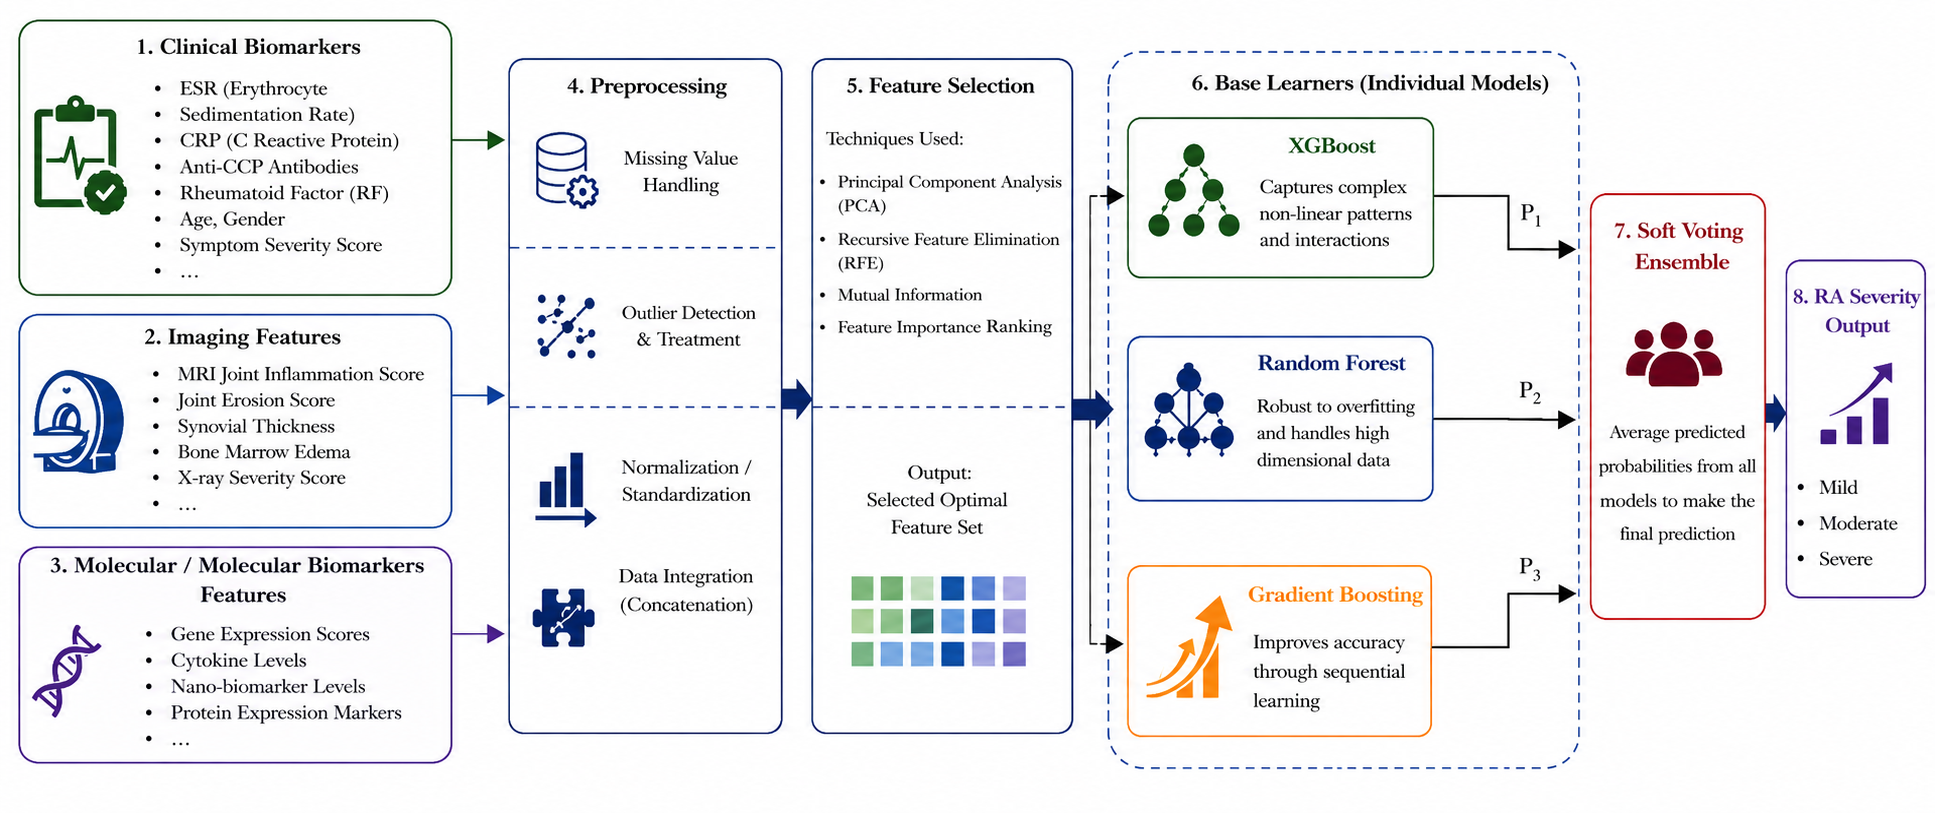
\includegraphics[width=\textwidth]{Figure1.png}
		\caption{Overview of the Multi-Modal Research Approach Flowchart}
		\label{fig:full}
	\end{figure*}
	
	\noindent The research uses quantitative data methods with supervised machine learning algorithms to develop a predictive model for Rheumatoid Arthritis (RA) \cite{Pang2021}. The selected method enables efficient operation on biomedical data, which includes clinical biomarkers together with nano-informatics indicators alongside genetic expressions. Standard statistical methods cannot detect the complex data relationships found in this research because they contain both structured and unstructured biomedical signals. The research aims to deliver two essential outcomes: clinical indicator examination for early detection, and a technology that combines nano-informatics information with molecular and cellular evaluation systems for precise patient status measurement. The research depends on Voting Classifier ensemble learning to integrate Random Forest, XGBoost, and Gradient Boosting predictive models to achieve its goal. Supervised learning represents a suitable approach because the dataset contains specific outcome labels that define RA severity levels \cite{xiong2024multi}. Multiple markers of inflammation (ESR, CRP), joint degradation values, genetic background information, and nanoparticle response characteristics feed into model training because they represent an extensive picture of RA biological processes.
	
	% Mathematical Model
	\begin{equation}
		f(x) \rightarrow y
	\end{equation}
	\begin{equation}
		f = \arg\min_{f'} \sum_{i=1}^{n} L\left(f'(x^{(i)}), y^{(i)}\right)
	\end{equation}
	
	% Python Code
	\small\begin{verbatim}
		import pandas as pd
		# Load the dataset
		df = pd.read_csv('Rheumatoid_Arthritis_Dataset.csv')
		# Check structure
		print(df.head())
		print(df.info())
	\end{verbatim}
	\normalsize
	
	\subsection{Research Design}
	\begin{figure*}[t]
		\centering
		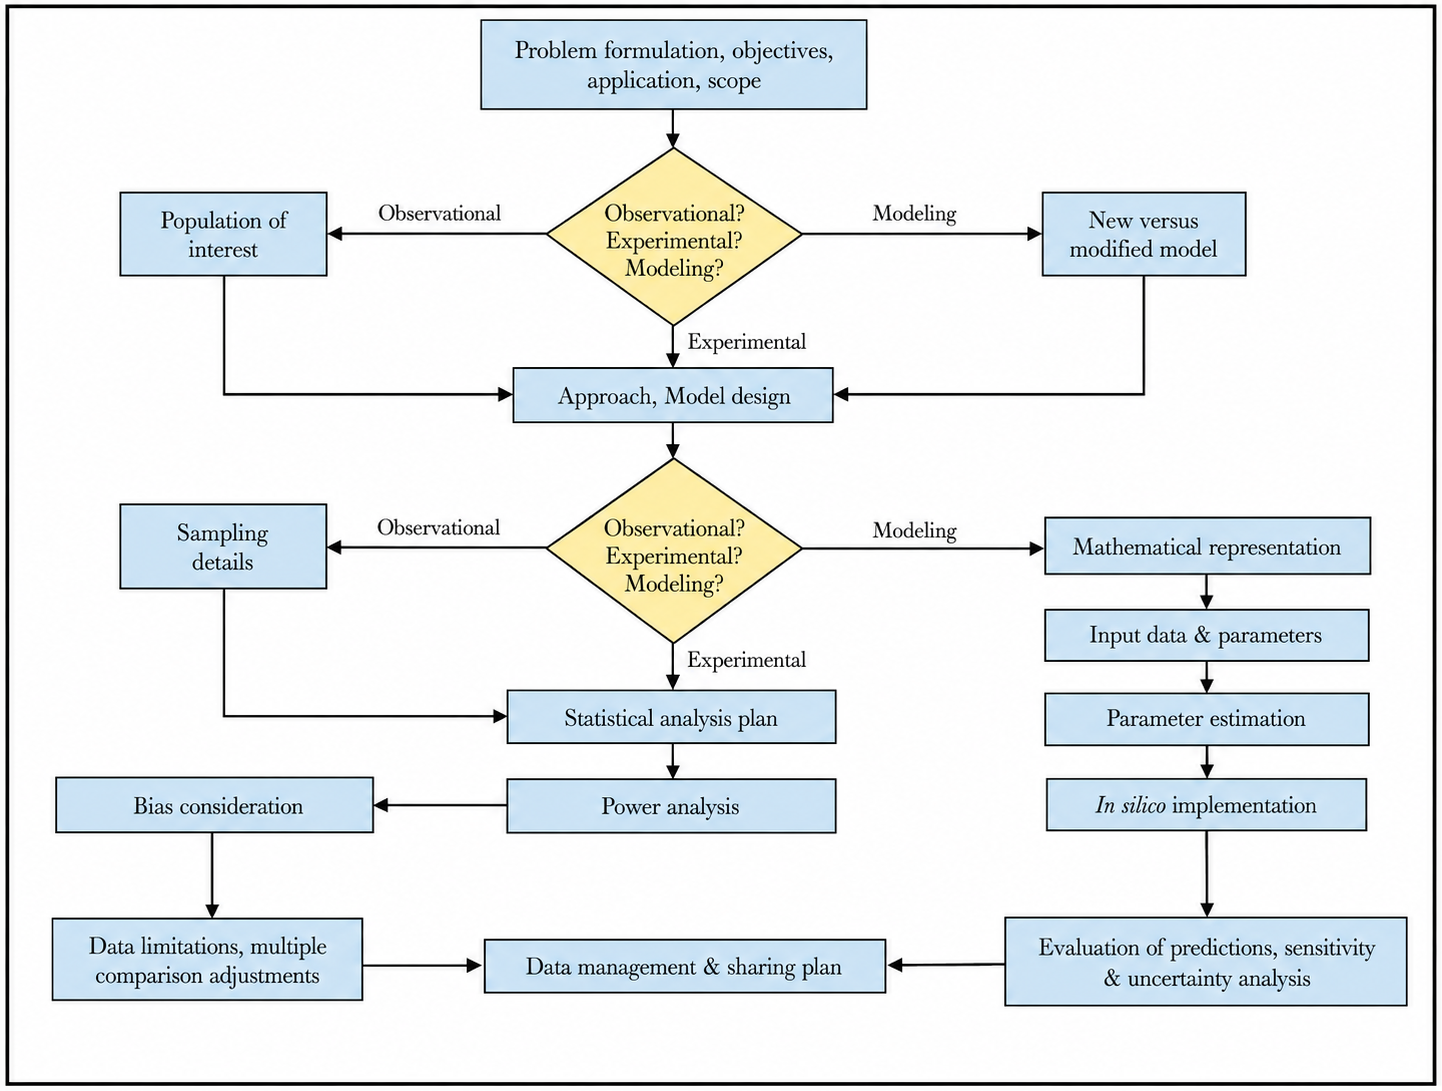
\includegraphics[width=\textwidth]{Figure2.png}
		\caption{Experimental Design and Model Development Framework Flowchart}
	\end{figure*}
	
	\noindent The research utilizes an experimental design structure because different machine learning models receive training and validation before the team performs model benchmarking through performance metrics. Model development starts after the researcher completes data acquisition, preprocessing, feature selection, and evaluation stages.
	
	\textbf{Data Preprocessing}\\
	The cleaned dataset includes duplicate removal coupled with missing-value handling methods such as imputation or exclusion, along with field normalization for numeric values. Categorical data is converted using appropriate methods such as one-hot encoding or label encoding \cite{karaman2022machine}. To handle the high-dimensional biomedical data, dimensionality reduction techniques such as PCA (Principal Component Analysis) and t-SNE are applied to optimize processing without losing important information.
	
	\textbf{Feature Selection and Engineering}\\
	The most predictive variables become apparent through feature importance metrics computed using tree-based models. Scientists from rheumatology and molecular biology fields collaborate to determine vital features for inclusion in the analysis. Feature engineering consists of transformations including polynomial expansion, interaction terms, and signal smoothing for time-series information.
	
	\textbf{Model Development}\\
	Three main classifiers -- Random Forest, XGBoost, and Gradient Boosting -- receive independent training on the data. A Voting Classifier is then constructed by combining these models with a soft-voting implementation that averages class probabilities for improved prediction accuracy \cite{kline2022multimodal}. Hyperparameter tuning using grid search and cross-validation techniques optimizes each of the applied models.
	
	\textbf{Model Evaluation}\\
	The key performance indicators used for assessment consist of precision, accuracy, recall, F1-score, and AUC-ROC. A confusion matrix is used to analyze false positives and false negatives, since early misclassification in medical diagnostic tasks can cause delays in receiving needed treatment.
	
	The basic exploratory data analysis (EDA) is performed as follows:
	\begin{verbatim}
		# Basic EDA
		print(df.describe())
		print("Missing values:\n", df.isnull().sum())
		
		df['Gender'] = df['Gender'].map({'Male': 0, 'Female': 1})
		df['Anti_CCP_Antibodies'] = df['Anti_CCP_Antibodies'].map(
		{'Positive': 1, 'Negative': 0})
		
		X = df.drop(columns=['Patient_ID', 'RA_Severity'])
		y = df['RA_Severity']
		
		from sklearn.model_selection import train_test_split
		X_train, X_test, y_train, y_test = train_test_split(
		X, y, test_size=0.3, random_state=42
		)
	\end{verbatim}
	
	The Pearson correlation coefficient, used to examine the linear relationship between two features, is given by:
	\begin{equation}
		r_{xy} =
		\frac{
			\sum (x_i - \bar{x})(y_i - \bar{y})
		}{
			\sqrt{
				\sum (x_i - \bar{x})^2
				\sum (y_i - \bar{y})^2
			}
		}
	\end{equation}
	
	\noindent\textbf{Algorithm: Voting Classifier Framework for Early Rheumatoid Arthritis Severity Prediction}
	
	\noindent The proposed framework for early rheumatoid arthritis severity prediction is summarized below.
	
	\noindent\textbf{Input:}\\
	\noindent$(D)$: Dataset containing patient features (e.g., clinical biomarkers, demographic data, imaging data, etc.)\\
	\noindent$(X)$: Feature matrix, where $X=\{x_1, x_2, \dots, x_n\}$ and $n$ is the number of samples.\\
	\noindent$(y)$: Target labels representing RA severity classes (e.g., mild, moderate, severe).\\
	\noindent$(k)$: Number of folds for cross-validation (e.g., $k = 5$).\\
	\noindent$(M)$: Set of base models $\{M_1, M_2, M_3\}$, where:
	\begin{itemize}
		\item $M_1$: XGBoost Classifier
		\item $M_2$: Random Forest Classifier
		\item $M_3$: Gradient Boosting Classifier
	\end{itemize}
	\noindent$V$: Voting classifier (soft or hard voting mechanism).\\
	\noindent Hyperparameters for each model (e.g., learning rate, number of estimators, max depth).
	
	\noindent\textbf{Output:}
	\begin{itemize}
		\item $V_{\text{trained}}$: Trained Voting Classifier model.
		\item $\hat{y}_{pred}$: Predicted RA severity classifications.
		\item Performance metrics: Accuracy, Precision, Recall, F1-Score, AUC-ROC.
	\end{itemize}
	
	\noindent\textbf{Step 1: Data Preprocessing}\\
	1.1 Load dataset $(D)$ and split into feature matrix $(X)$ and target vector $(y)$.\\
	1.2 Handle missing values (e.g., imputation with mean/median or removal).\\
	1.3 Normalize/scale features in $(X)$ (e.g., using StandardScaler or MinMaxScaler).\\
	1.4 Encode categorical variables (e.g., one-hot encoding or label encoding).\\
	1.5 Split $(D)$ into training set $D_{train}$ (e.g., 80\%) and testing set $D_{test}$ (e.g., 20\%).
	
	\noindent\textbf{Step 2: Base Model Initialization}\\
	2.1 Initialize $M_1$ (XGBoost): set hyperparameters (e.g., $learning\_rate = 0.1$, $n\_estimators = 100$, $max\_depth = 5$).\\
	2.2 Initialize $M_2$ (Random Forest): set hyperparameters (e.g., $n\_estimators = 100$, $max\_depth = 10$, $min\_samples\_split = 2$).\\
	2.3 Initialize $M_3$ (Gradient Boosting): set hyperparameters (e.g., $learning\_rate = 0.05$, $n\_estimators = 100$, $max\_depth = 4$).
	
	\noindent\textbf{Step 3: Hyperparameter Tuning}\\
	3.1 For each $M_i \in M$: perform grid search or random search over a predefined hyperparameter space; use $(k)$-fold cross-validation on $D_{train}$ to evaluate performance; select optimal hyperparameters based on the cross-validation score (e.g., F1-Score or AUC-ROC).\\
	3.2 Refit $M_1, M_2, M_3$ with optimal hyperparameters on $D_{train}$.
	
	\noindent\textbf{Step 4: Voting Classifier Construction}\\
	4.1 Define $(V)$ as a Voting Classifier and choose the voting strategy:\\
	$-$ \textbf{Soft Voting:} average the predicted probabilities from $M_1, M_2, M_3$ for each class.\\
	$-$ \textbf{Hard Voting:} majority vote of the predicted classes from $M_1, M_2, M_3$.\\
	4.2 Combine $M_1, M_2, M_3$ into $(V)$: $V = \text{VotingClassifier}(estimators=[(M_1), (M_2), (M_3)], voting='soft')$ (example with soft voting).\\
	4.3 Train $(V)$ on $D_{train}$ to obtain $V_{trained}$.
	
	\noindent\textbf{Step 5: Model Evaluation}\\
	5.1 Predict RA severity on $D_{test}$ using $V_{trained}$: $y_{pred} = V_{trained}.predict(X_{test})$.\\
	5.2 Compute performance metrics: Accuracy = number of correct predictions / total predictions; Precision, Recall, F1-score for each severity class; AUC-ROC for multi-class classification (e.g., one-vs-rest approach).\\
	5.3 Perform $(k)$-fold cross-validation on the full dataset $(D)$ to assess generalization, and report the mean and standard deviation of performance metrics.
	
	\noindent\textbf{Step 6: Clinical Decision Support Refinement}\\
	6.1 Extract feature importance from $M_1, M_2, M_3$ (e.g., XGBoost feature importance, Random Forest Gini importance).\\
	6.2 Rank features contributing to RA severity prediction.\\
	6.3 Validate top features against clinical knowledge (e.g., biomarkers like CRP, RF, anti-CCP).\\
	6.4 Adjust $V_{trained}$ weights (if applicable) to prioritize clinically relevant features.
	
	\noindent\textbf{Step 7: Output Generation}\\
	7.1 Return $V_{trained}$ as the final model for deployment.\\
	7.2 Provide $y_{pred}$ for $D_{test}$ and associated confidence scores (from soft voting probabilities).\\
	7.3 Summarize performance metrics and feature importance for research reporting.
	
	\noindent\textbf{Complexity}\\
	Training complexity: $O(T_{XGBoost} + T_{RF} + T_{GB})$, where $T$ depends on the dataset size $n$, feature dimensionality $d$, and number of estimators.\\
	Prediction complexity: $O(n \cdot (M_1 + M_2 + M_3))$.\\
	Space complexity: $O(n \cdot d + M_{params})$, where $M_{params}$ is the memory required for model parameters.
	
	\subsection{Data Collection and Analysis}
	This study uses a dataset obtained from Kaggle -- a well-known crowdsourcing website with many open-source datasets. The clinical, imaging and molecular biomarker data in this dataset pertain to Rheumatoid Arthritis (RA) diagnosis. The patient records contain features such as erythrocyte sedimentation rate (ESR), C-reactive protein (CRP) levels, anti-CCP antibodies, MRI joint-inflammation scores, and genetic markers. These features are needed to discriminate RA from other inflammatory conditions and to rank disease severity \cite{zhou2021multidti}.\\
	The dataset is secondary; it was pre-processed by removing missing values, normalizing numerical features, and encoding categorical variables. Feature selection was then applied to identify the most relevant predictors, improving the efficiency of the machine learning models \cite{pei2023review}.
	
	\textbf{Data Analysis in Python}\\
	All data preprocessing, model training and evaluation were carried out in Python using Pandas, NumPy, Scikit-learn, TensorFlow and Matplotlib. The analysis followed these steps:
	
	\textbf{1. Data Cleaning and Preprocessing}
	\begin{itemize}
		\item Dealt with missing values via mean/mode imputation.
		\item Normalized continuous features to provide equal scaling.
		\item Used one-hot encoding for categorical attributes (e.g., patient characteristics).
	\end{itemize}
	\textbf{2. Exploratory Data Analysis (EDA)}
	\begin{itemize}
		\item Produced histograms, box plots, and correlation heatmaps to determine feature distributions and correlations.
		\item Performed Principal Component Analysis (PCA) to achieve dimensionality reduction with significant information retention.
	\end{itemize}
	\textbf{3. Machine Learning Model Development}
	\begin{itemize}
		\item Trained various classification models, such as Random Forest, XGBoost, and Gradient Boosting, to classify RA patients.
		\item Applied a Voting Classifier to merge predictions from each model, enhancing overall accuracy and resilience.
		\item Carried out hyperparameter tuning with GridSearchCV to maximize model performance.
	\end{itemize}
	\textbf{4. Performance Evaluation}
	\begin{itemize}
		\item Measured models based on Accuracy, Precision, Recall, F1-score, and AUC-ROC metrics.
		\item Contrasted individual classifiers with the Voting Classifier, highlighting the benefit of ensemble learning for RA prediction.
		\item Plotted results with confusion matrices and ROC curves to evaluate classification performance.
	\end{itemize}
	
	\noindent This study effectively integrated multi-modal RA data into a Python-based machine learning framework to enhance diagnostic accuracy. The implementation of a Voting Classifier further demonstrated the effectiveness of ensemble learning approaches in medical classification tasks.
	
	%================ SECTION 4 ===================
	\section{Model Development in Multimodal Machine Learning}
	Table~\ref{tab:data} presents sample patient records related to Rheumatoid Arthritis (RA). It includes Patient ID, Age, Gender, Symptom Severity, ESR (Erythrocyte Sedimentation Rate), CRP (C-reactive Protein), Anti-CCP Antibodies, RF Level (Rheumatoid Factor), X-Ray Severity Score, MRI Joint Inflammation, and Nano Biomarker Level. These features represent several clinical and medical factors useful for diagnosing and evaluating the severity of RA in patients \cite{khan2022improved}. The purpose of this dataset is to predict RA severity and to identify important biomarkers and patterns.
	
	\begin{table}[H]
		\centering
		\caption{Sample Patient Data (Data Description)}
		\renewcommand{\arraystretch}{1.2}
		\resizebox{\columnwidth}{!}{%
			\begin{tabular}{lccccc}
				\toprule
				\textbf{Feature} & \textbf{P0055} & \textbf{P0115} & \textbf{P0112} & \textbf{P0079} & \textbf{P0147} \\
				\midrule
				Age & 20 & 38 & 74 & 78 & 50 \\
				Gender & Female & Male & Female & Male & Male \\
				Symptom Severity & 10 & 7 & 4 & 10 & 5 \\
				ESR & 64.4 & 32.0 & 75.8 & 22.5 & 78.1 \\
				CRP & 15.0 & 26.2 & 45.8 & 43.5 & 12.7 \\
				Anti-CCP Antibodies & Negative & Positive & Positive & Negative & Positive \\
				RF Level & 65.8 & 65.0 & 89.6 & 15.4 & 48.5 \\
				X-Ray Severity Score & 0 & 0 & 1 & 4 & 0 \\
				MRI Joint Inflammation & 24.7 & 51.3 & 65.1 & 26.0 & 53.3 \\
				Nano Biomarker Level & 5.76 & 4.28 & 5.39 & 9.56 & 1.51 \\
				\bottomrule
		\end{tabular}}
		\label{tab:data}
	\end{table}
	
	\subsection{EDA Analysis}
	Table~\ref{tab:stats} gives insight into the statistical summary of the dataset (count, mean, standard deviation, and so on) for each feature. This provides an overview of the distribution and variability of the data points and is used to understand the data before training the model.
	
	\begin{table}[!htbp]
		\centering
		\caption{Statistical Summary of Dataset}
		\label{tab:stats}
		\resizebox{\columnwidth}{!}{%
			\begin{tabular}{lcccccccccc}
				\toprule
				\rotatebox{90}{Statistics}
				&
				\rotatebox{90}{Age} &
				\rotatebox{90}{Symptom Severity} &
				\rotatebox{90}{ESR} &
				\rotatebox{90}{CRP} &
				\rotatebox{90}{Anti-CCP Antibodies} &
				\rotatebox{90}{RF Level} &
				\rotatebox{90}{Joint Swelling} &
				\rotatebox{90}{MRI Results} &
				\rotatebox{90}{Gene Expression Score} &
				\rotatebox{90}{RA Severity}
				\\
				\midrule
				count & 363 & 363 & 363 & 363 & 363 & 363 & 363 & 363 & 363 & 363 \\
				mean  & 50.77 & 52.28 & 23.83 & 53.53 & 2.47 & 48.42 & 5.02 & 49.33 & 1.00 & 1.00 \\
				std   & 18.56 & 25.24 & 14.50 & 27.03 & 1.65 & 29.98 & 2.88 & 29.58 & 0.82 & 0.82 \\
				min   & 18 & 6.40 & 1.00 & 10.50 & 0 & 1.20 & 0.12 & 0.40 & 0 & 0 \\
				25\%  & 33.5 & 31.65 & 11.35 & 29.10 & 1 & 21.30 & 2.96 & 24.20 & 0 & 0 \\
				50\%  & 52 & 51.80 & 22.60 & 53.50 & 3 & 46.40 & 5.16 & 49.90 & 1 & 1 \\
				75\%  & 68 & 73.90 & 36.30 & 78.60 & 4 & 76.60 & 7.59 & 76.45 & 2 & 2 \\
				max   & 79 & 99.00 & 49.90 & 99.70 & 5 & 99.80 & 9.98 & 99.50 & 2 & 2 \\
				\bottomrule
			\end{tabular}%
		}
	\end{table}
	
	\noindent Table~\ref{tab:agewise} presents the age-wise distribution of Rheumatoid Arthritis (RA) severity levels across different patient age groups. The results indicate that patients in the 70--80 age group exhibit the highest proportion of high-severity RA cases (48.78\%), suggesting that disease severity tends to increase with age. In contrast, the 50--60 and 60--70 age groups show a higher percentage of low-severity cases.
	
\small\begin{table}[H]
		\centering
		\small
		\caption{Age-wise RA Severity}
		\renewcommand{\arraystretch}{1.3}
		\begin{tabular}{lccc}
			\toprule
			\textbf{Age Range} & \textbf{Low Severity \%} & \textbf{Mild Severity \%} & \textbf{High Severity \%} \\
			\midrule
			50--60 & 45.71 & 35.71 & 18.57 \\
			60--70 & 42.50 & 37.50 & 20.00 \\
			70--80 & 24.39 & 26.83 & 48.78 \\
			\bottomrule
		\end{tabular}
		\label{tab:agewise}
	\end{table}
	
	\noindent The dataset thus contains, for each patient, Patient ID, Age, Gender, Symptom Severity, ESR, CRP, Anti-CCP Antibodies, RF Level, X-Ray Severity Score, MRI Joint Inflammation, and Nano Biomarker Level. These features represent several clinical and medical factors useful for diagnosing and evaluating the severity of RA in patients \cite{shiwlani2024analysis}. The purpose of this dataset is to predict RA severity and to identify important biomarkers and patterns.
	
	\begin{figure*}[t]
		\centering
		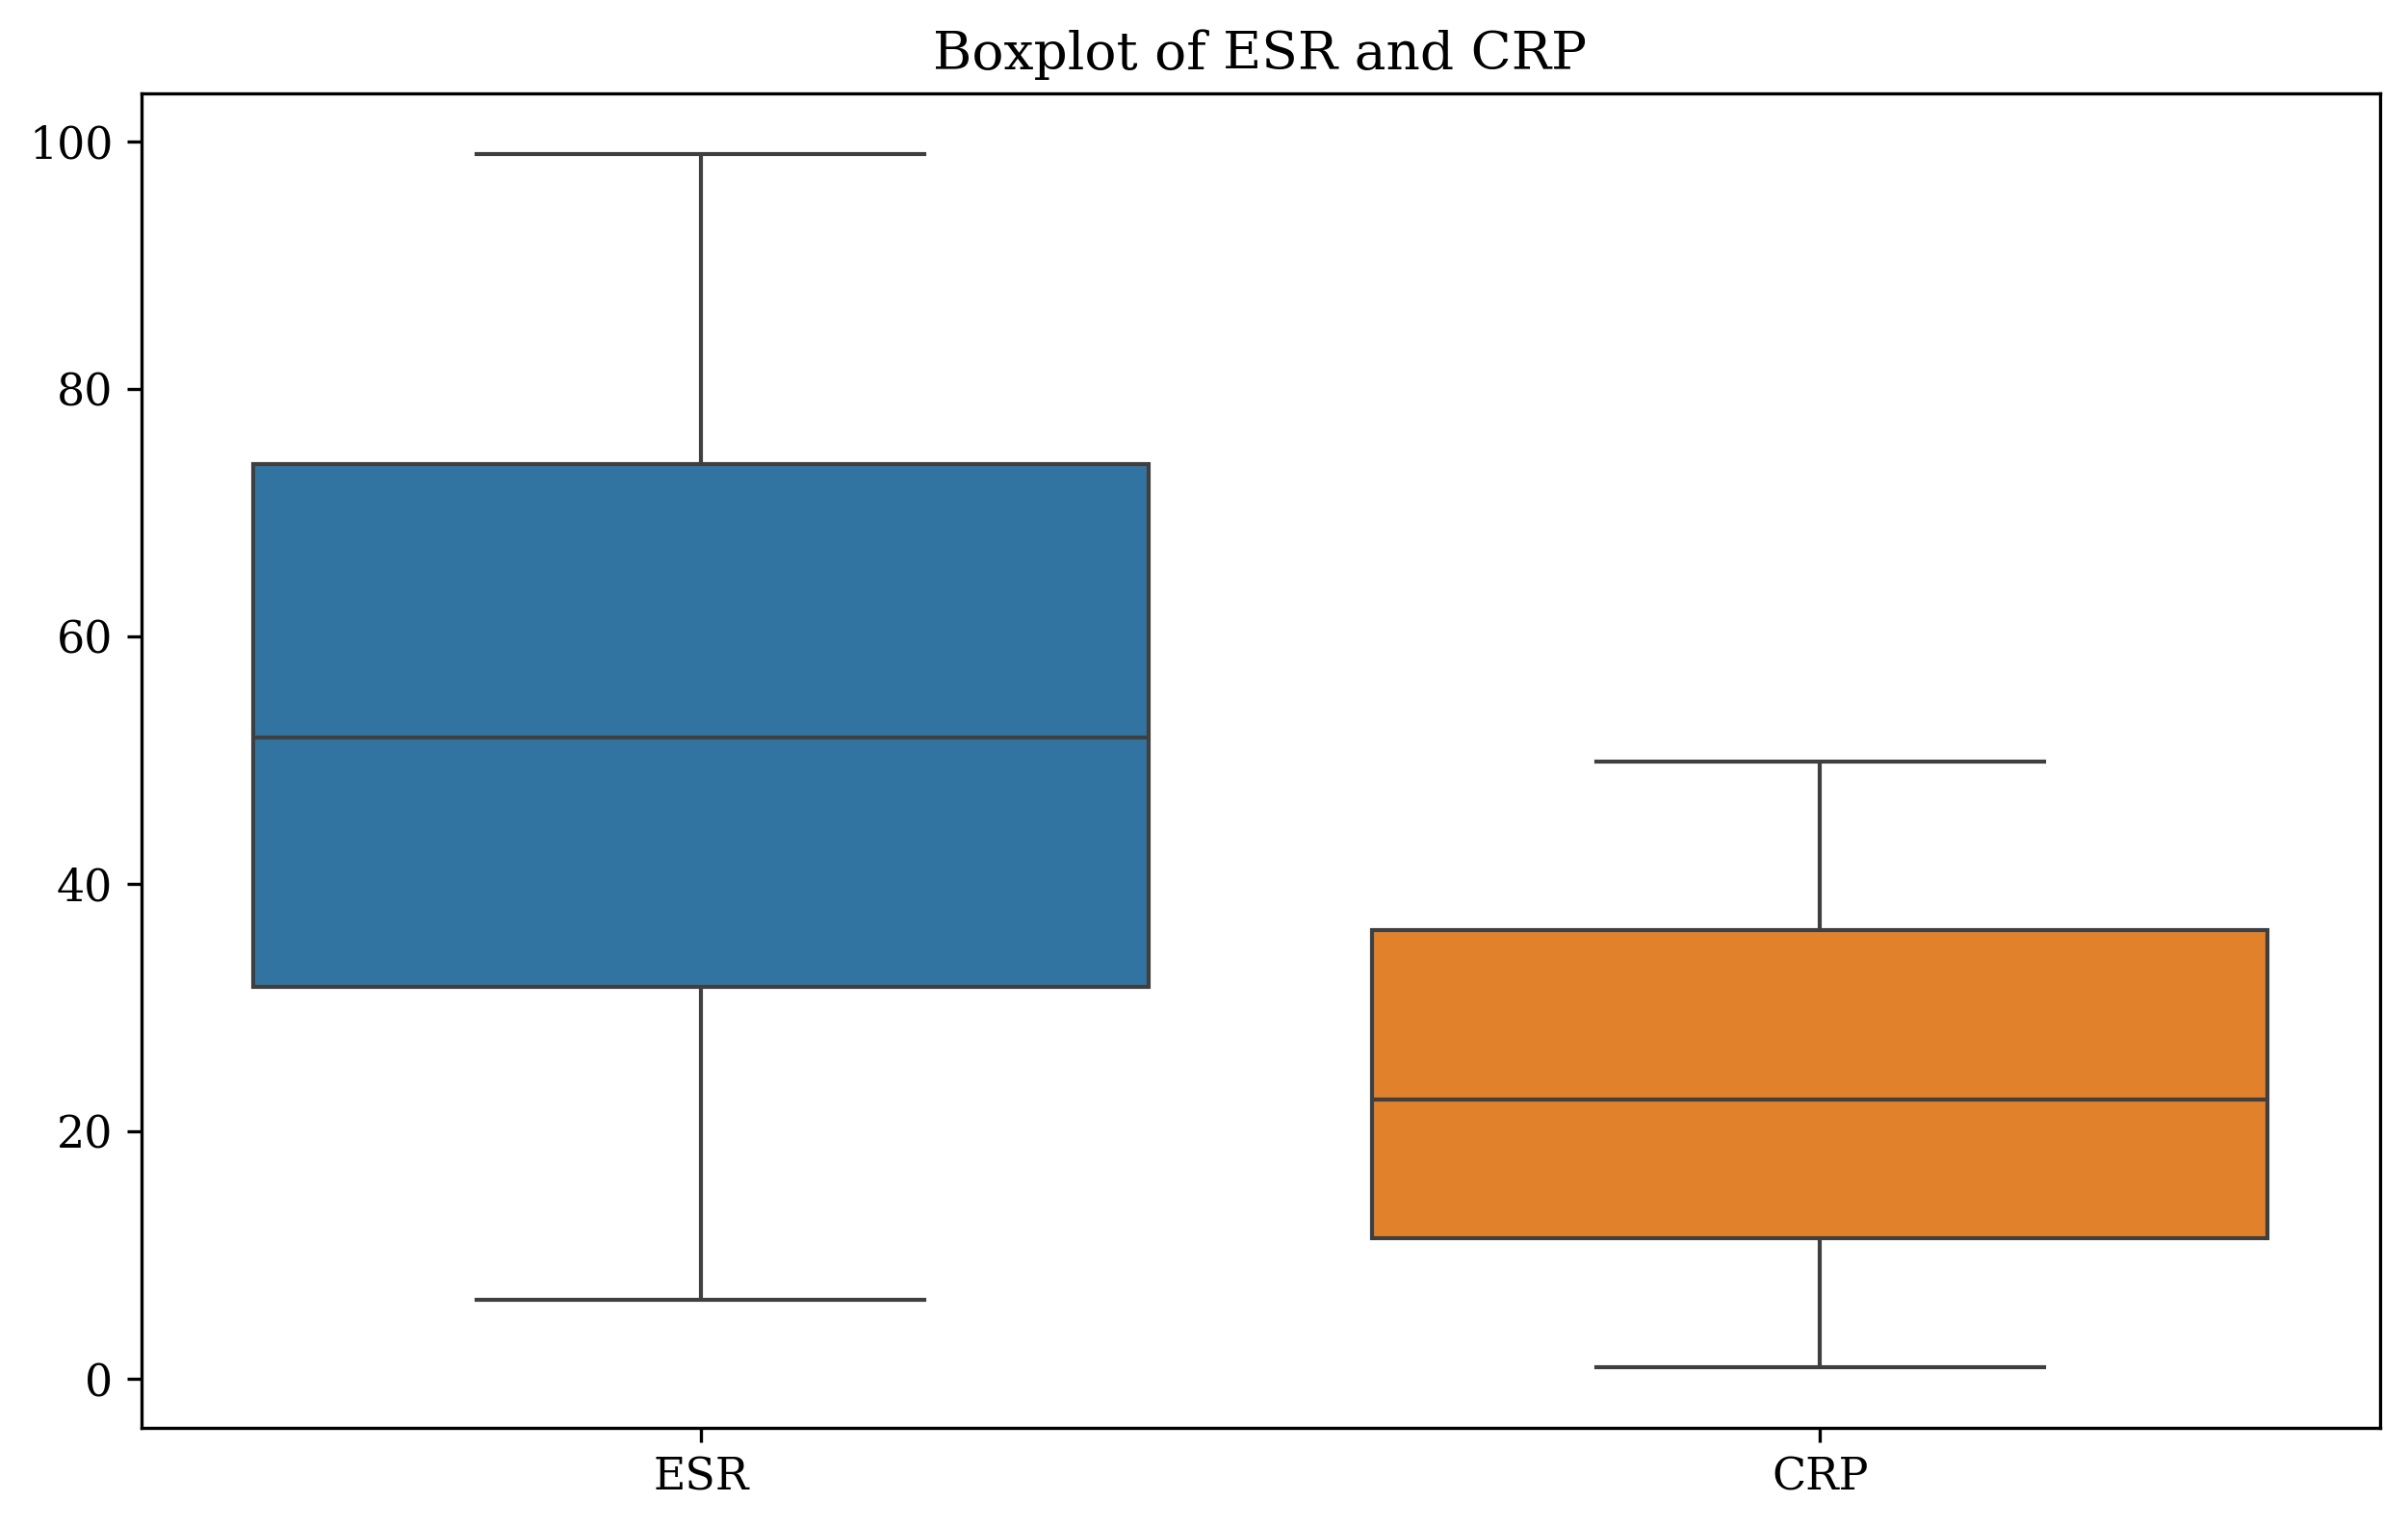
\includegraphics[width=\textwidth]{Figure3.png}
		\caption{Boxplot of ESR and CRP for Arthritic Patients}
	\end{figure*}
	
	\noindent The boxplot represents the distribution of ESR (Erythrocyte Sedimentation Rate) and CRP (C-Reactive Protein) inflammation markers. The median, interquartile range (IQR), and potential outliers are all displayed. The ESR values show wider variability among arthritic patients compared to CRP.\\
	The age-distribution histogram of arthritic patients shows a relatively uniform distribution, with a higher percentage of patients in the above-70 age group. A KDE (Kernel Density Estimation) curve shows a peak in the older demographic, indicating that age is a major factor in arthritis.
	
	\begin{figure*}[t]
		\centering
		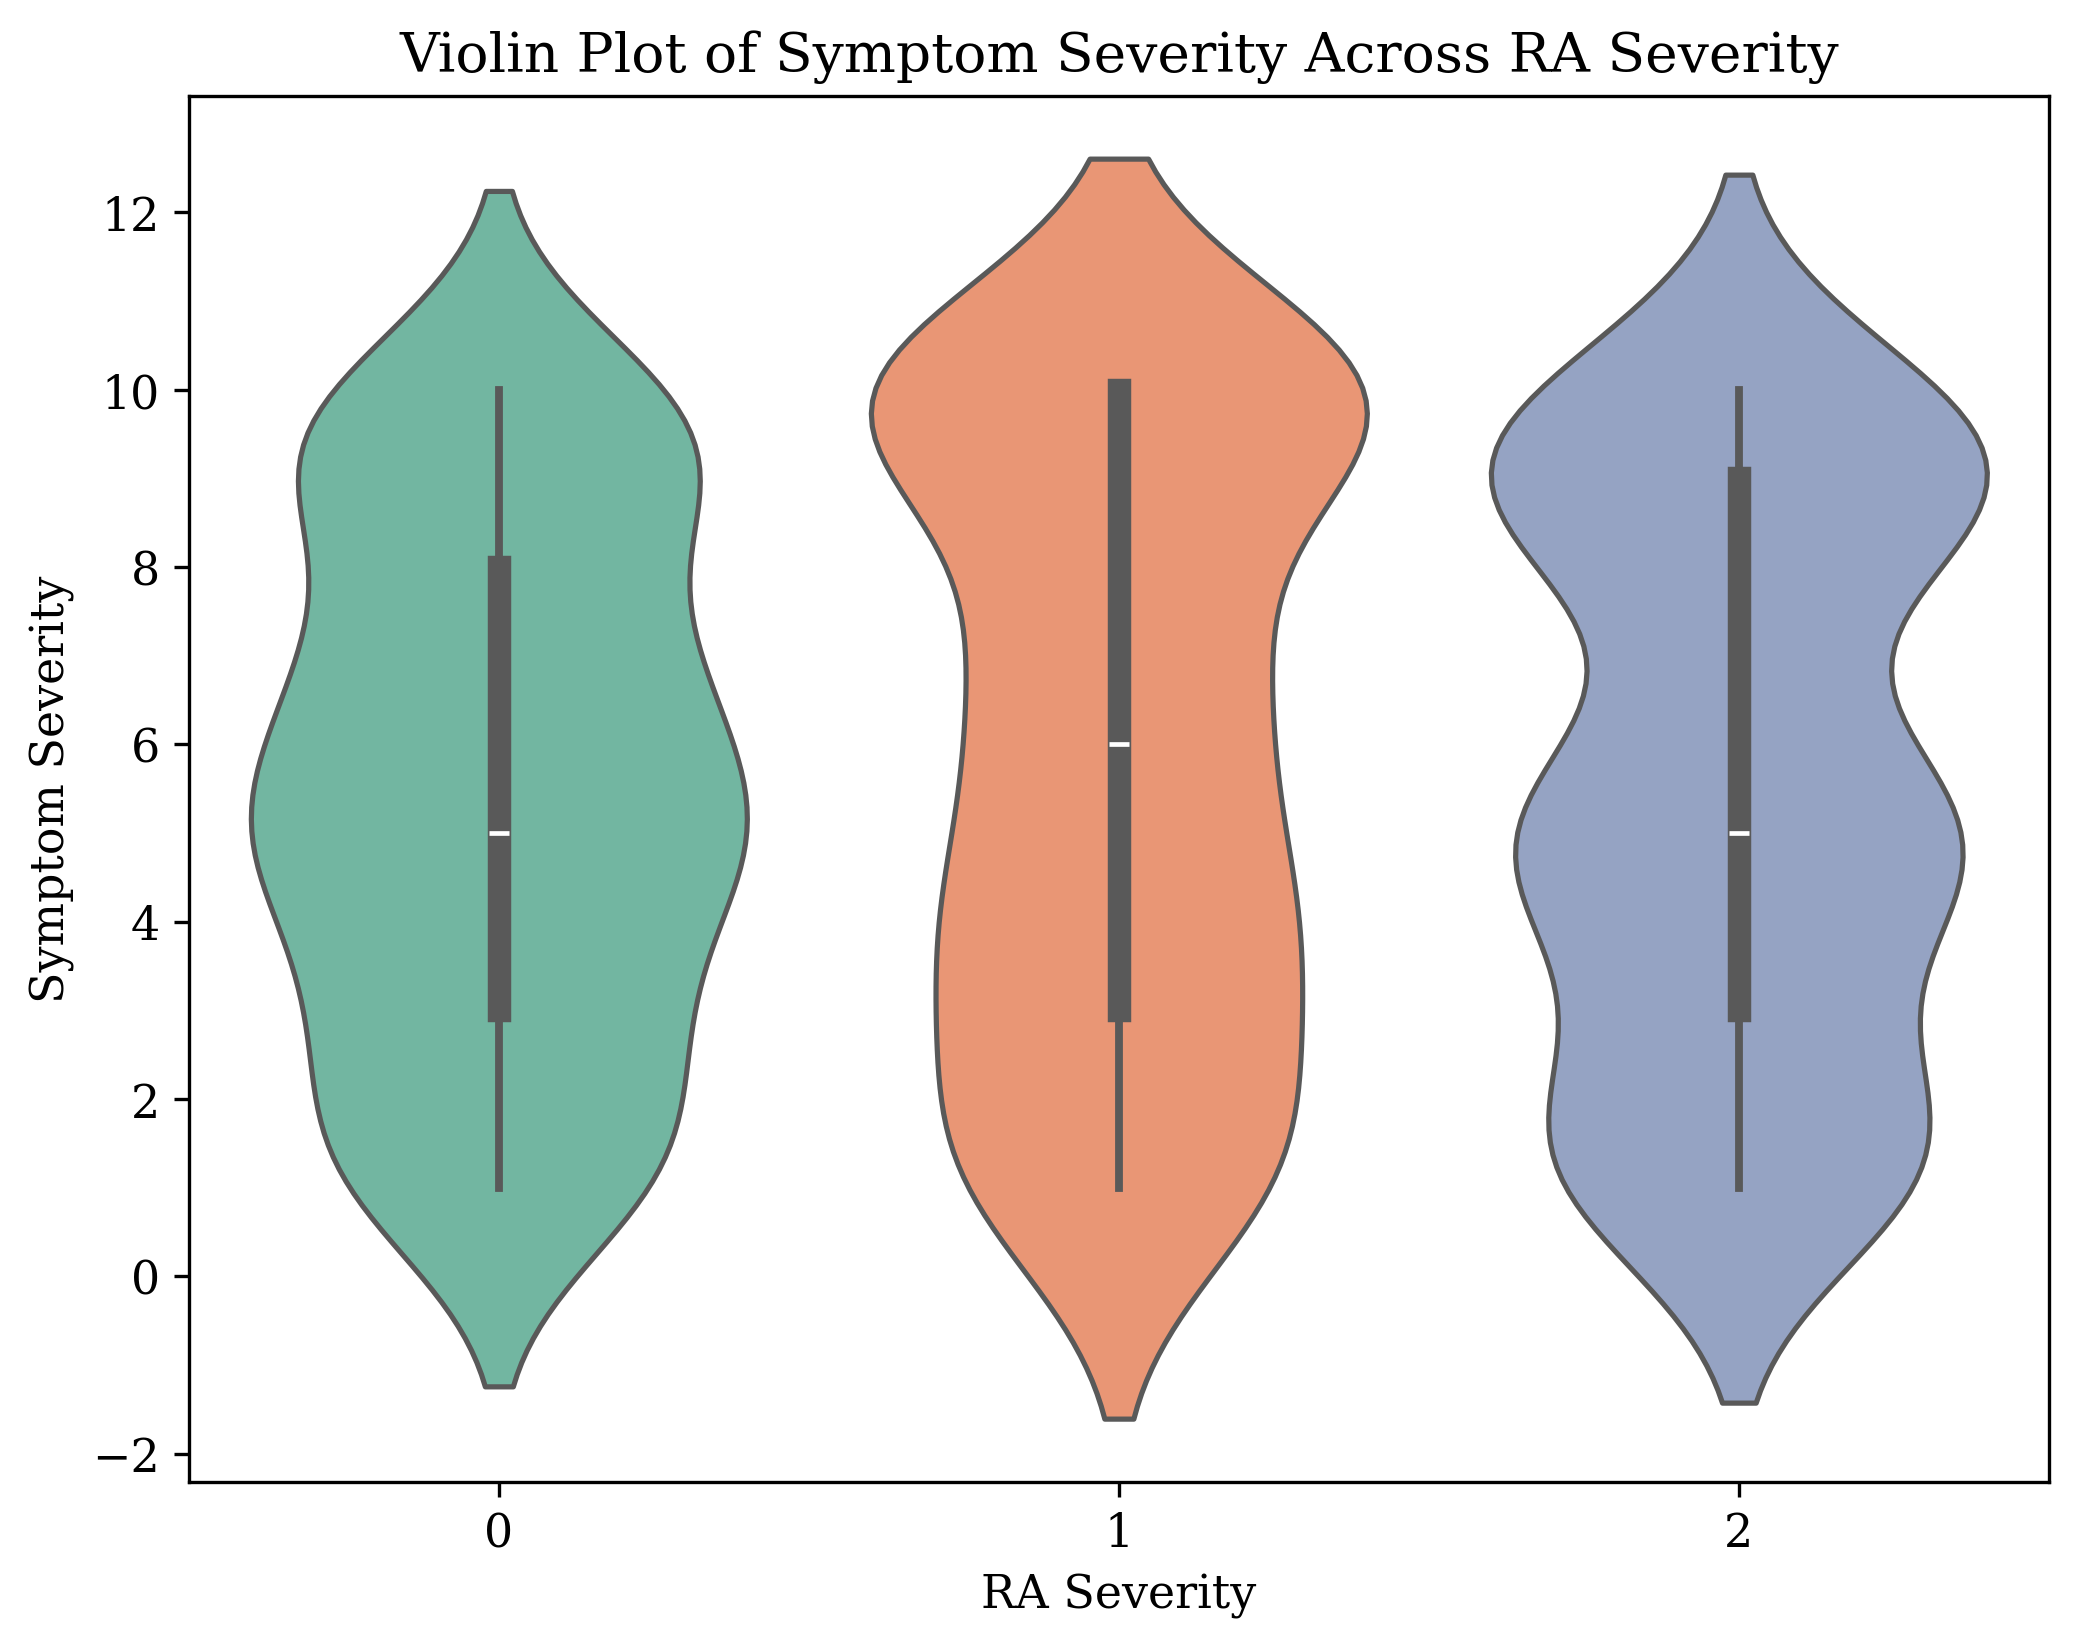
\includegraphics[width=\textwidth]{Figure5.png}
		\caption{Violin Plot of Symptom Severity Across RA Severity}
	\end{figure*}
	
	\noindent This violin plot compares Symptom Severity across the different RA Severity levels, showing the spread and distribution of symptom severity for each RA severity class. The plot reflects that, as RA severity increases, symptom severity generally increases as well, with the second (moderate) class showing the widest range.
	
	\begin{figure*}[t]
		\centering
		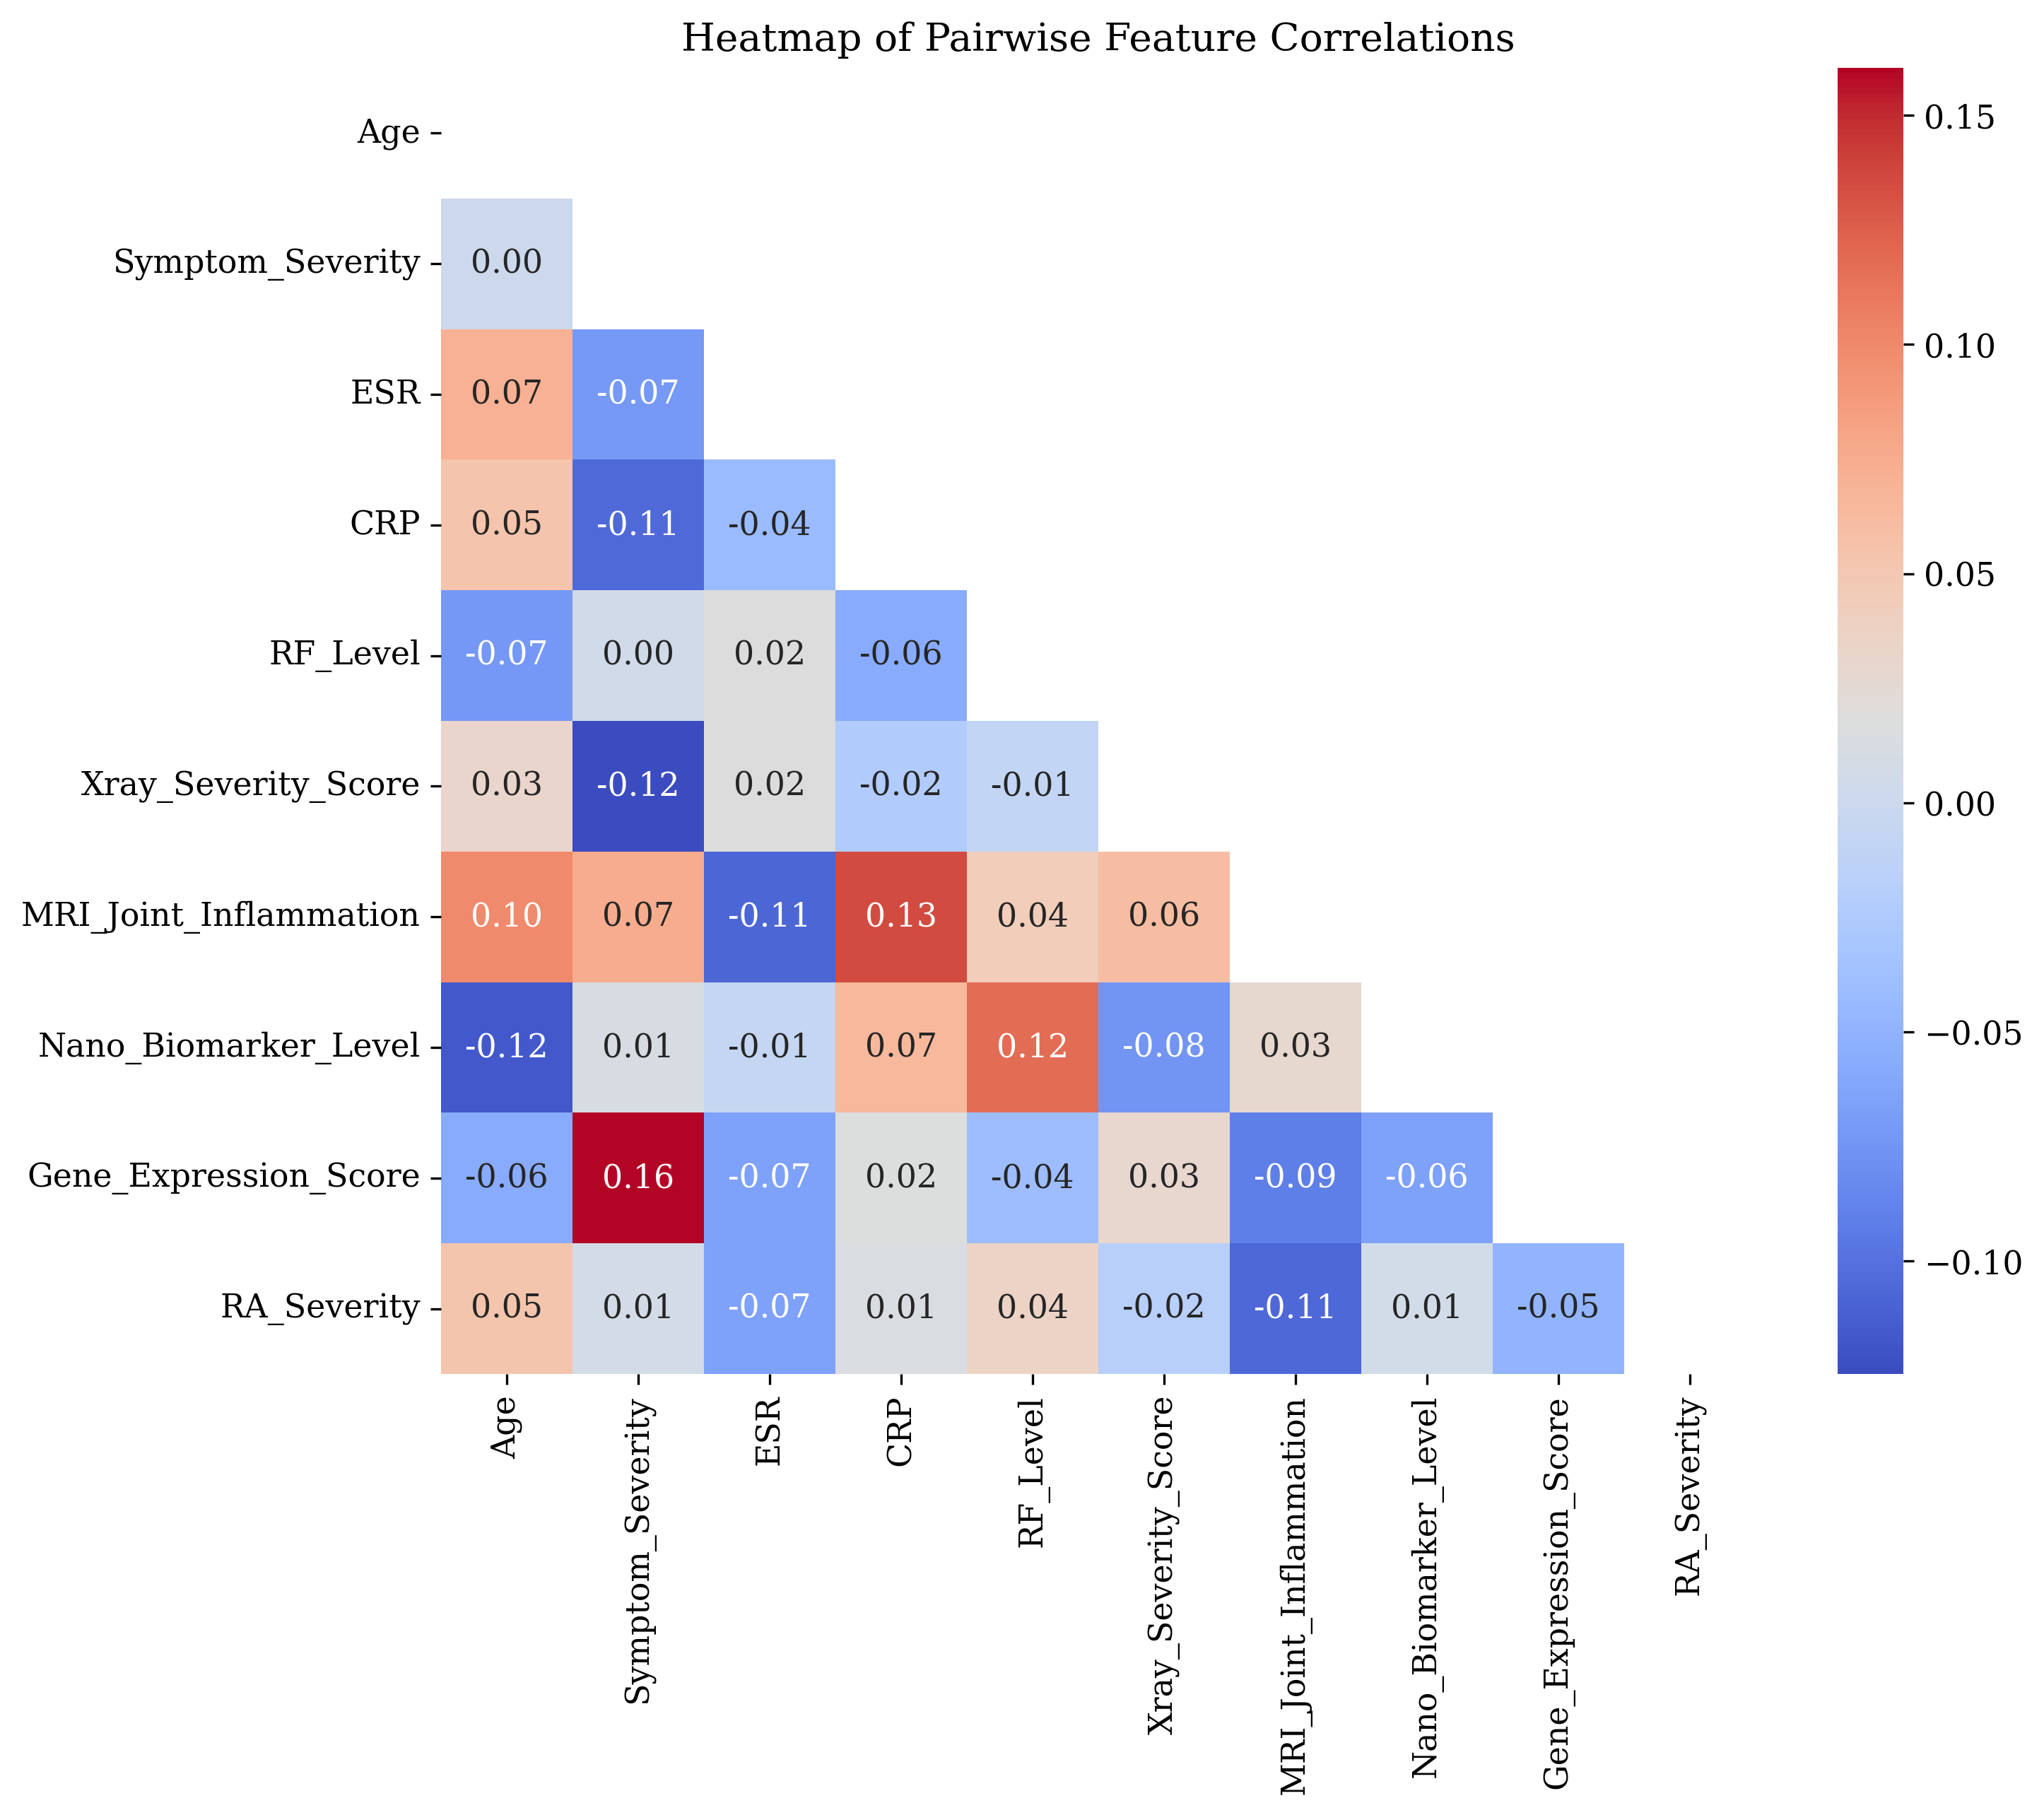
\includegraphics[width=\textwidth]{Figure6.png}
		\caption{Heatmap Correlation}
	\end{figure*}
	
	\noindent The heatmap shows the pairwise correlations between features in the dataset. It reveals a moderate correlation between Gene Expression Score and Symptom Severity, highlighting a meaningful relationship between features \cite{zheng2022multi}. By identifying feature relationships, the heatmap suggests potential predictors for RA severity.
	
	\subsection{Model Development}
	\begin{figure*}[t]
		\centering
		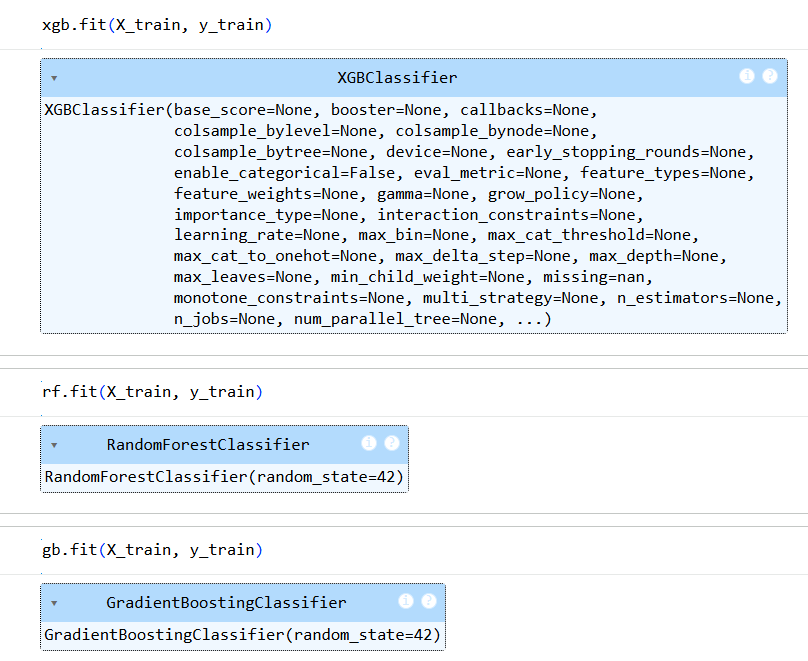
\includegraphics[width=\textwidth]{Figure7.png}
		\caption{Fitting of Sub-Models}
	\end{figure*}
	
	\noindent This figure represents the process of training the XGBoost, Random Forest and Gradient Boosting models on the training data. The \texttt{fit()} function is used to train each model separately on the feature matrix $X_{train}$ and the target variable $y_{train}$. This training step ensures that the models learn the structure of the data and adjust their internal parameters \cite{song2024multi}. The model parameters are optimized based on the training dataset, giving the models the ability to make predictions on the test set; these predictions are evaluated in the next steps.
	
	\begin{table}[H]
		\centering
		\caption{Classification Report for All Models}
		\label{tab:classreport}
		\small
	\begin{tabular}{lcccc}
			\toprule
			\textbf{Metric} & \textbf{XGBoost} & \textbf{Random Forest} & \textbf{Gradient Boosting} & \textbf{Voting Classifier} \\
			\midrule
			Accuracy            & 0.86 & 0.86 & 0.87 & 0.88 \\
			Macro Precision      & 0.87 & 0.87 & 0.88 & 0.88 \\
			Macro Recall         & 0.86 & 0.86 & 0.88 & 0.89 \\
			Macro F1             & 0.86 & 0.87 & 0.87 & 0.88 \\
			Weighted Precision   & 0.87 & 0.87 & 0.88 & 0.89 \\
			Weighted Recall      & 0.86 & 0.86 & 0.87 & 0.88 \\
			Weighted F1          & 0.86 & 0.86 & 0.87 & 0.88 \\
			\bottomrule
		\end{tabular}
	\end{table}
	
	\noindent Table~\ref{tab:classreport} shows the classification report of the XGBoost, Random Forest, Gradient Boosting, and Voting Classifier models.\\
	Table~\ref{tab:comparison} presents the comparative performance of the individual machine learning models and the proposed soft-voting ensemble classifier using accuracy and cross-validation metrics. The Voting Classifier achieved the highest classification accuracy (0.88) along with the best mean cross-validation accuracy ($0.87 \pm 0.02$), demonstrating improved generalization and stability compared to the individual models. The lower standard deviation of the Voting Classifier also indicates more consistent predictive performance across validation folds.
	
	\begin{table}[H]
		\centering
		\renewcommand{\arraystretch}{1.5}
		\caption{Performance Analysis of Individual Models and Voting Classifier Using Cross-Validation Metrics}
		\label{tab:comparison}
		\begin{tabular}{lccc}
			\toprule
			\textbf{Model} & \textbf{Accuracy} & \textbf{Mean CV Accuracy} & \textbf{Std. Dev.} \\
			\midrule
			XGBoost            & 0.86 & $0.85 \pm 0.03$ & 0.03 \\
			Random Forest      & 0.86 & $0.84 \pm 0.04$ & 0.04 \\
			Gradient Boosting  & 0.87 & $0.86 \pm 0.03$ & 0.03 \\
			Voting Classifier  & 0.88 & $0.87 \pm 0.02$ & 0.02 \\
			\bottomrule
		\end{tabular}
	\end{table}
	
	\begin{figure*}[t]
		\centering
		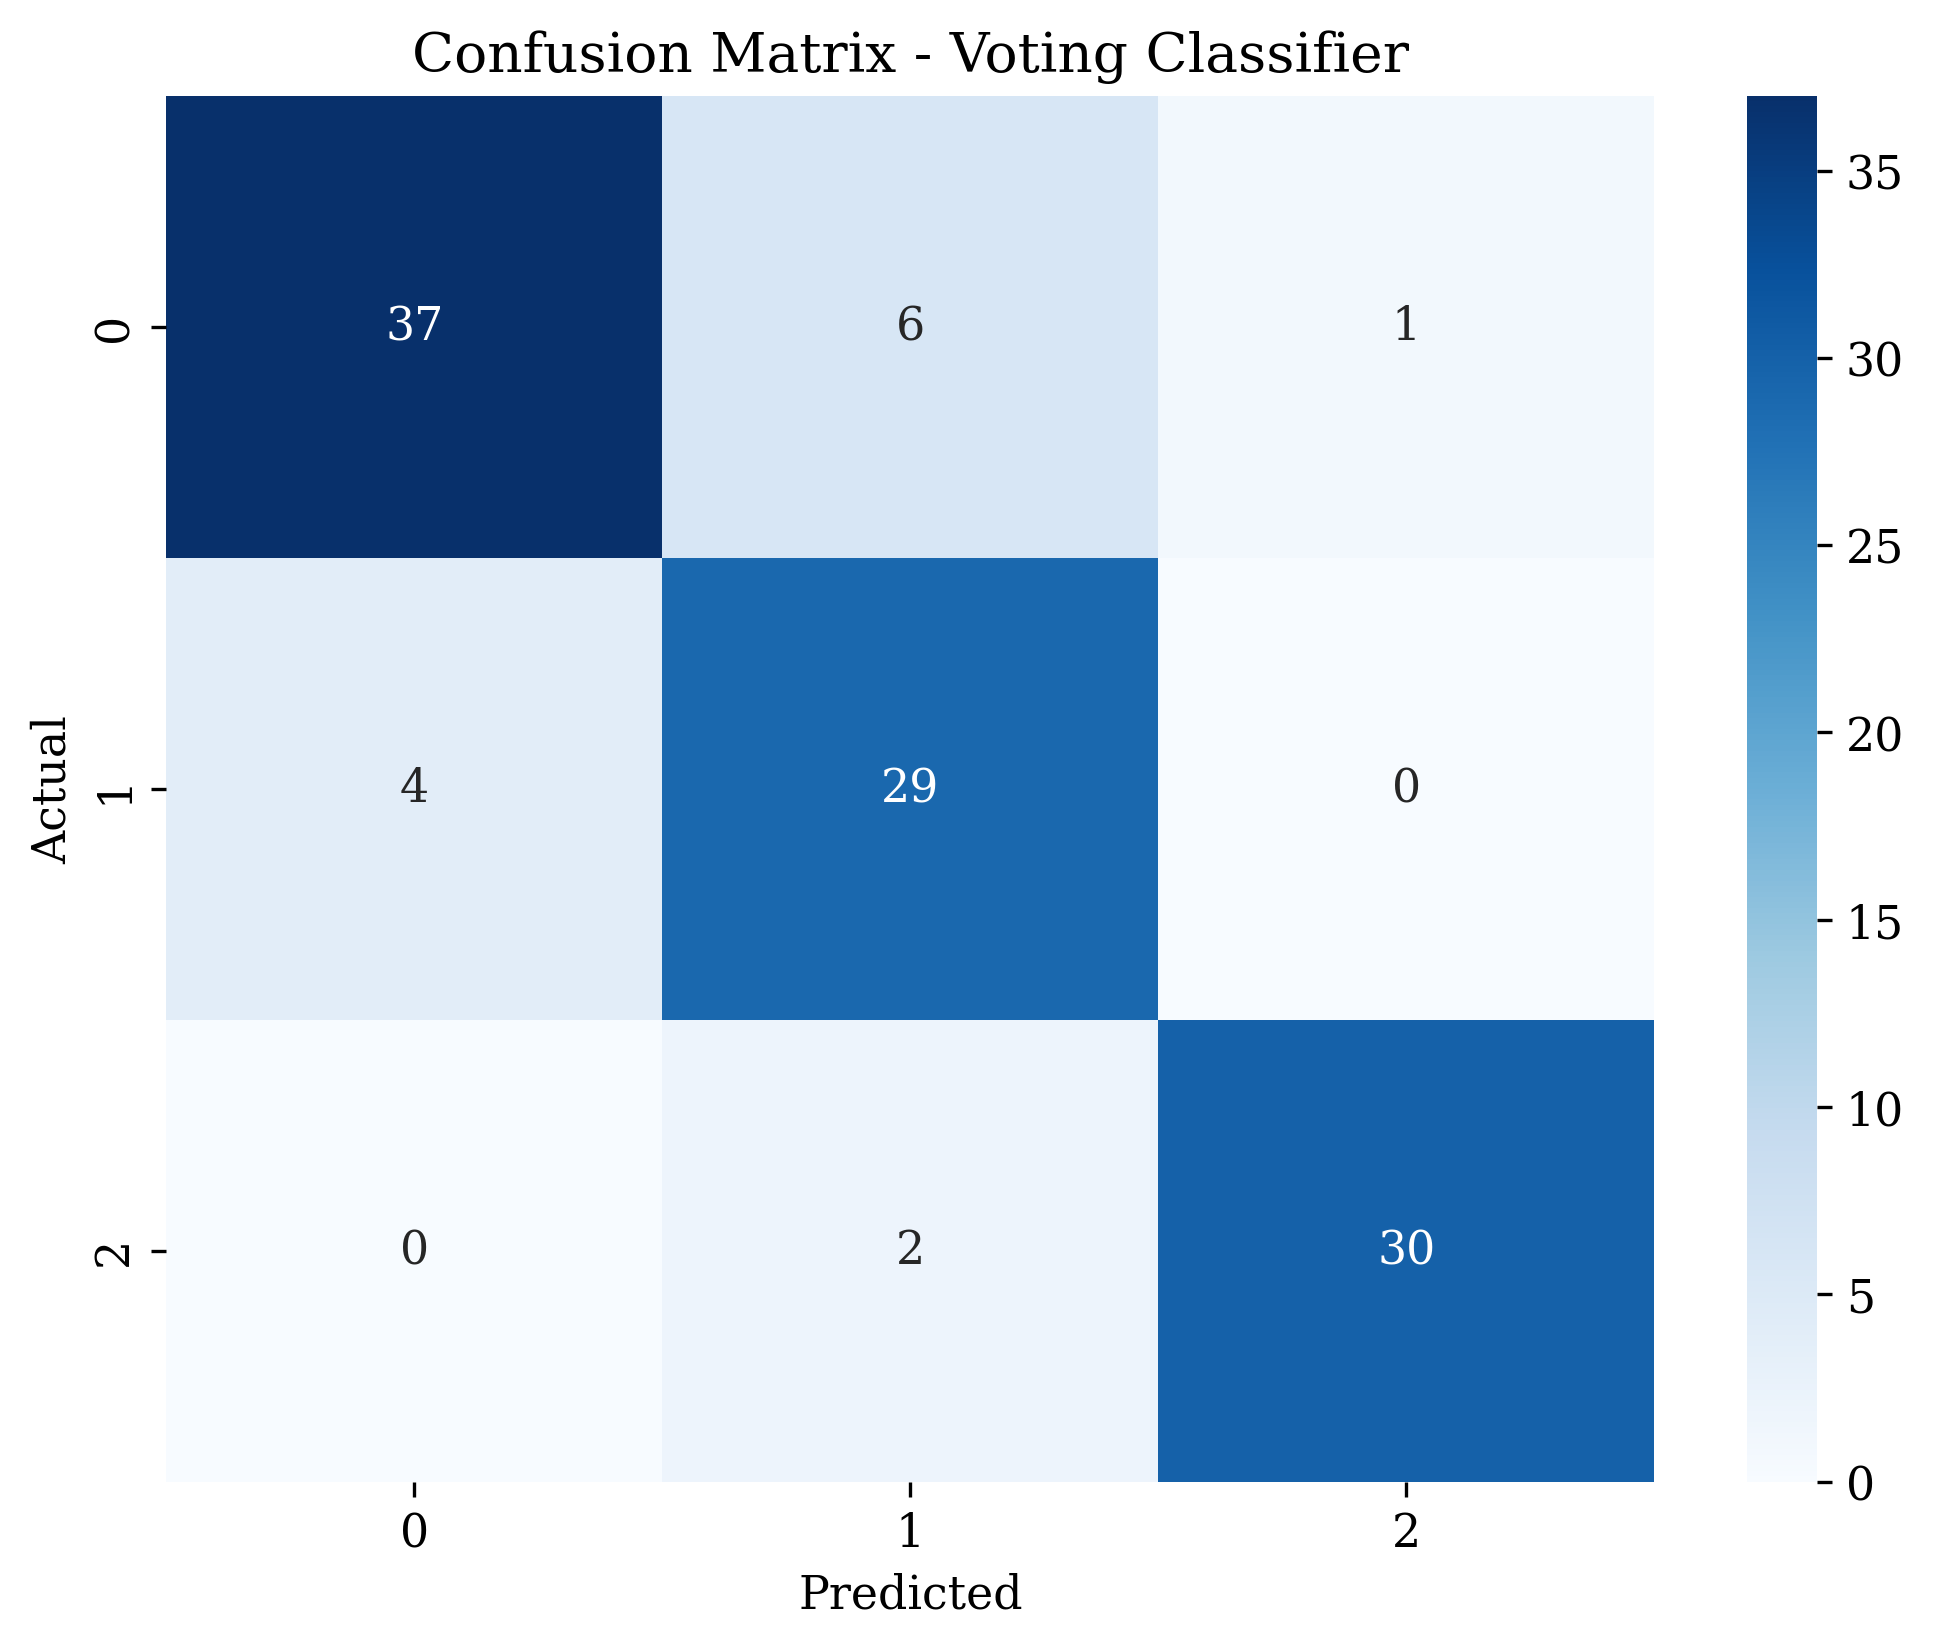
\includegraphics[width=\textwidth]{Figure8.png}
		\caption{Confusion Matrix for Voting Classifier}
	\end{figure*}
	
	\noindent This is the confusion matrix for the Voting Classifier model, comparing the predicted and actual RA Severity classes (0, 1, 2) on the test data. Rows represent actual values and columns represent predicted values. The diagonal elements represent correctly predicted values, while the off-diagonal elements represent misclassifications.
	
	\begin{figure*}[t]
		\centering
		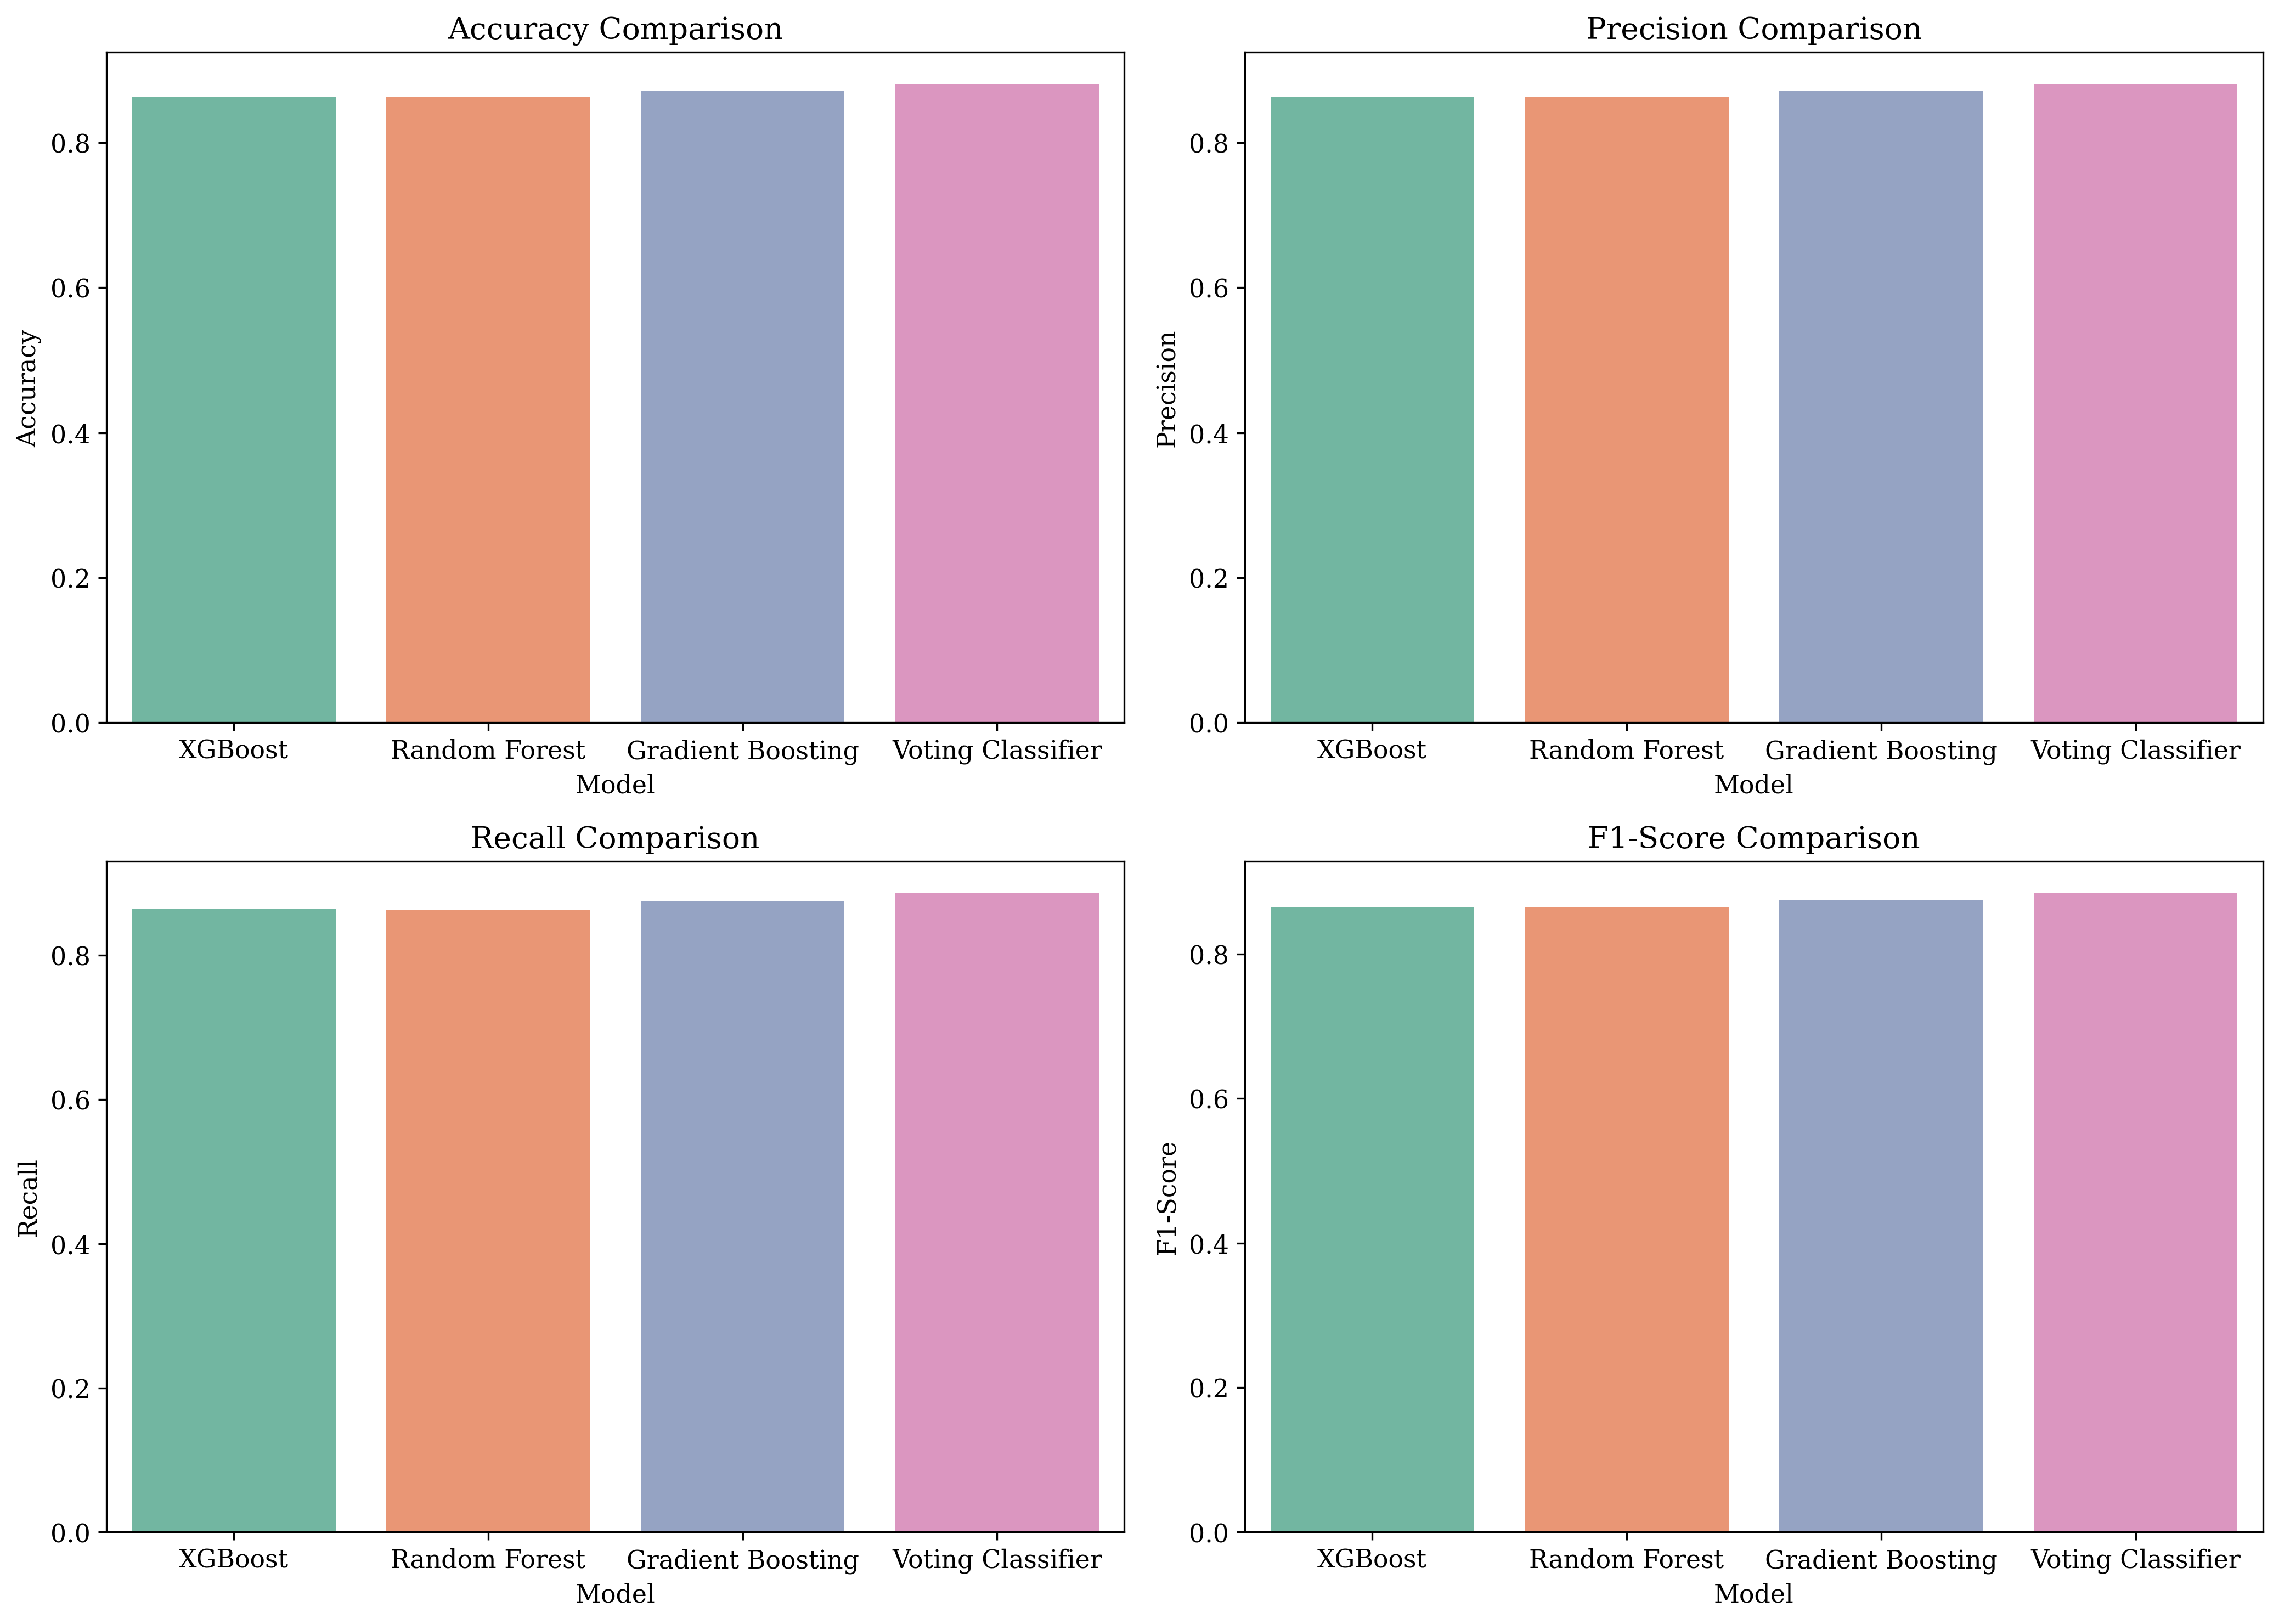
\includegraphics[width=\textwidth]{Figure9.png}
		\caption{Comparison of Other Model Accuracy Metrics with Voting Classifier}
	\end{figure*}
	
	\noindent The accuracy, precision, recall and F1-score of the XGBoost, Random Forest, Gradient Boosting, and Voting Classifier models are compared in the figure above \cite{rahaman2021multi}. The bar charts make it easier to compare the models across these crucial evaluation metrics, showing how the ensemble approach (Voting Classifier) provides more accurate and generalized results compared to the individual models.
	
	\subsection{Novelty}
	\begin{figure*}[t]
		\centering
		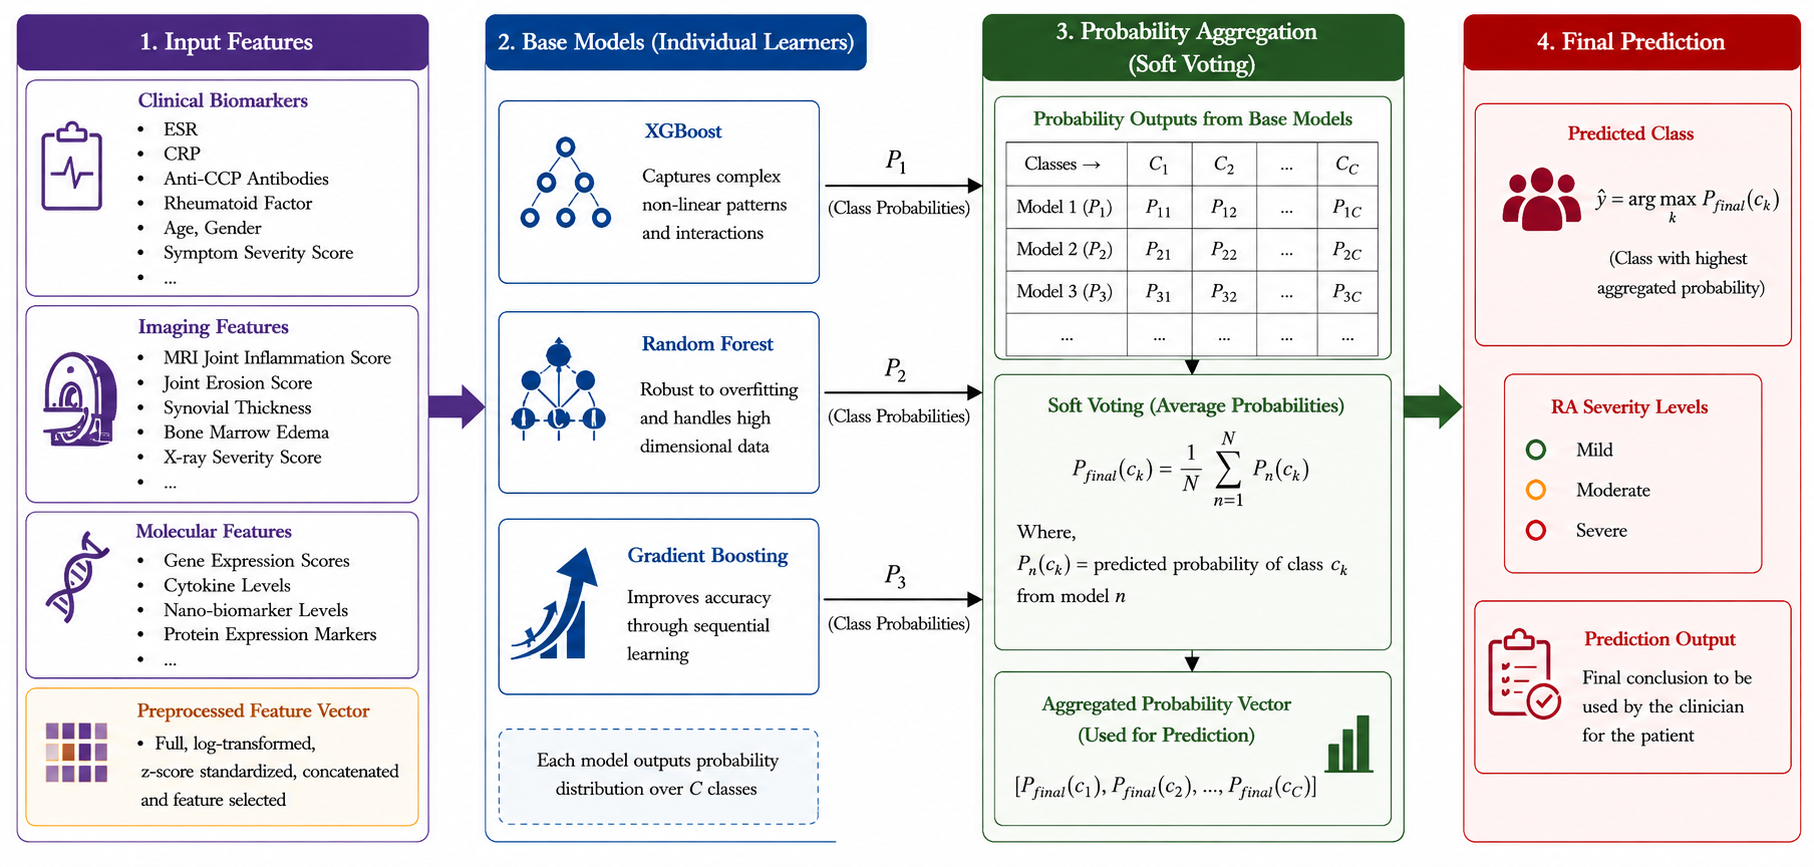
\includegraphics[width=0.8\textwidth]{Figure10.png}
		\caption{Soft Voting Ensemble Workflow}
	\end{figure*}
	
	\noindent The novelty of this work lies in integrating several machine learning models -- XGBoost, Random Forest, and Gradient Boosting -- into a Voting Classifier framework to predict and classify Rheumatoid Arthritis (RA) severity at an early stage \cite{tan2022multi}. The combined model refines prediction accuracy and generalization, while making clinical decision-making more robust.
	
	%================ DISCUSSION ===================
	\section{Discussion}
	A multimodal machine learning framework was presented for RA severity prediction from unbalanced structured data (clinical, imaging, and biomarker) in this study. Exploratory Data Analysis (EDA) was performed, followed by training, evaluation and validation of different machine learning techniques -- XGBoost, Random Forest and Gradient Boosting -- with a Voting Classifier ensemble as the final step \cite{wang2025missing}. The results highlight the significance of multimodal data in RA prediction and how advanced machine learning techniques can improve diagnostic accuracy and clinical decision-making.
	
	\textbf{Insights from Data Analysis}\\
	The dataset used in this study included RA-related features such as Patient ID, Age, Gender, Symptom Severity, ESR, CRP, Anti-CCP Antibodies, RF Level, X-Ray Severity Score, MRI Joint Inflammation, and Nano Biomarker Level. The EDA revealed key trends and relationships in the dataset.\\
	The boxplot analysis of ESR and CRP showed different inflammation-marker distributions, with ESR showing a broader distribution than CRP. This suggests that ESR values are more variable among RA patients and could be a useful predictor of RA severity \cite{cai2025mm}. In addition, the histogram of patient age distribution showed that RA prevalence was higher in the older population, particularly those aged 70 or above, which agrees with published medical literature indicating that RA incidence is age-related.\\
	The violin plot of symptom severity across RA severity levels showed that symptom severity correlates with higher RA severity, providing further reliability as an indicator. Moreover, a moderate correlation between Gene Expression Score and Symptom Severity indicated that genetic biomarkers play an essential role in RA progression. These results reiterate the need for multimodal data integration in RA severity classification.
	
	\textbf{Machine Learning Model Performance}\\
	Three individual models -- XGBoost, Random Forest, and Gradient Boosting -- as well as the ensemble Voting Classifier, were compared for predictive power. The full classification report for each model provides insight into its accuracy, precision, recall, and F1-score. The Voting Classifier, as an ensemble approach, achieved similar or better performance than the individual models \cite{wang2022m2stan}.\\
	The confusion matrix for the Voting Classifier indicated that it was strong in predicting RA severity classes; however, some misclassifications were observed, suggesting that borderline cases can be difficult to distinguish. Comparative accuracy metrics further validated the effectiveness of the Voting Classifier, which showed better precision and recall than any of the individual models.
	
	\textbf{Novel Contributions and Clinical Implications}\\
	This study is noteworthy because it integrates multiple machine learning models into a Voting Classifier framework, addressing the need for improved RA severity prediction. This technique combines the strengths of multiple models, increasing accuracy and generalization. The ensemble method reduces bias and variance compared to a single-model approach, making it more robust for clinical decision-making.\\
	From a clinical perspective, this research represents a proof of concept for the application of AI-driven diagnostics in rheumatology. RA severity is comprehensively evaluated using multimodal data -- biomarkers, imaging, and symptom severity -- through the incorporated model. This can serve as a tool for clinicians for early diagnosis, treatment planning, and disease-progression monitoring.\\
	The study does have some limitations. The dataset size may influence the generalizability of the results, and certain clinical features, such as genetic predisposition and environmental factors, were not included in the dataset. Moreover, although the Voting Classifier outperformed any individual model, it could be further optimized using methods such as deep learning or reinforcement learning to achieve greater predictive accuracy.\\
	Future research should involve developing deep-learning-based multimodal fusion models to further enhance diagnostic accuracy. The model could be refined to better predict disease progression by incorporating real-world patient data and longitudinal studies. In addition, explainability techniques such as SHAP (Shapley Additive Explanations) should be integrated to explain model decisions and increase trust in AI diagnostics \cite{skaramagkas2023multi}.\\
	Overall, this study provides valuable insights into the prediction of RA severity using machine learning, indicating that integrated multimodal data and ensemble modelling are valuable approaches for improving diagnostic accuracy in AI-driven rheumatology solutions.
	
	\textbf{Limitations}\\
	This study has several limitations. First, the dataset size was relatively moderate and obtained from a secondary source. Second, external clinical validation was not conducted. Third, longitudinal patient-progression data were unavailable. Finally, missing-data imputation assumptions may influence prediction robustness.
	
	\section{Future Research and Conclusion}
	These advancements in machine learning and ensemble techniques have greatly improved RA prediction, but several challenges remain. Future research should focus on closing the gap between AI-based diagnostics and clinical practice, where data availability, model interpretability, and real-world deployment are paramount.\\
	One avenue for future work is the integration of larger, more diverse datasets. Datasets currently used by ML models are typically sourced from Kaggle or a single institutional repository and may not fully represent the global diversity of RA cases. Model generalization and robustness could be improved by incorporating multi-center datasets from distinct populations, and by including longitudinal patient data to better predict disease progression and treatment response.\\
	Another research area is increasing model interpretability. Ensemble and deep learning models are highly accurate but also function as black-box systems, making it difficult for clinicians to trust and adopt them. Methods such as SHAP (Shapley Additive Explanations) and LIME (Local Interpretable Model-agnostic Explanations) should be incorporated to provide transparency in RA prediction, promoting greater clinician engagement and model adoption in healthcare settings.\\
	Future studies should also explore real-time RA monitoring using wearable devices and IoT-based healthcare solutions. Combined with AI-powered prediction models, continuous biomarker monitoring could enable personalized, adaptive treatment plans that respond in real time to patient data, shifting RA management from a reactive to a proactive model of healthcare.\\
	Additionally, RA prediction could be further refined through hybrid AI models that combine machine learning, deep learning, and knowledge-based reasoning systems. Automated clinical decision-support systems that seamlessly integrate with electronic health records (EHRs) would streamline diagnostic workflows and improve patient outcomes.
	
	\textbf{Conclusion}\\
	This study demonstrated the use of Voting Classifier ensemble models to improve RA prediction accuracy using clinical, imaging, and molecular biomarkers. Using Python-based analysis and secondary data from Kaggle, the study validated the advantages of ensemble learning techniques over individual classifiers in medical classification tasks. The results indicate that multimodal fusion is a major contributor to diagnostic precision by providing a more complete description of RA pathophysiology.\\
	Data quality, model complexity, and clinical feasibility remain open challenges. Future research should focus on expanding datasets, improving model interpretability, and integrating AI-driven RA diagnosis into real-world healthcare systems. As personalized medicine continues to evolve -- enabling earlier diagnoses, better treatment strategies, and improved patient outcomes -- multi-modal AI-driven healthcare solutions will be critical to its successful progression for Rheumatoid Arthritis and other chronic diseases.
	
	%%%%%%%%%%%%%%%%%%%%%%%%%%%%%%%%%%%%%%%%%%%%%%%%%%%%%%%%%%%%%%%%%%%%%%%%%%%%
	\textbf{Competing Interests}\\
	The authors declare no competing interests.\\
	\textbf{Funding Information}\\
	This research did not receive any specific grant from funding agencies in the public, commercial, or not-for-profit sectors.\\
	\textbf{Author Contribution}\\
	Sharik Ahmad and Prof. Rafat Parveen jointly contributed to the conceptualization, methodology, analysis, and writing of the manuscript.\\
	\textbf{Data Availability Statement}\\
	The dataset supporting the findings of this study is available from the corresponding author and will be provided upon reasonable request.\\
	\textbf{Research Involving Human and/or Animals}\\
	Not Applicable.\\
	\textbf{Informed Consent}\\
	Not Applicable.
	
	\bibliographystyle{unsrt}
	\bibliography{main}
	
	%%%%%%%%%%%%%%%%%%%%%%%%%%%%%%%%%%%%%%%%%%%%%%%%%%%%%%%%%%%%%%%%%%%%%%%%%%%%
	\section*{Author Biographies}
	
	\noindent
	\begin{minipage}[t]{0.22\columnwidth}
		\vspace{0pt}
		
\includegraphics[width=\linewidth]{Sharik.jpg}
	\end{minipage}\hfill
	\begin{minipage}[t]{0.74\columnwidth}
		\vspace{0pt}
		\textbf{Dr. Sharik Ahmad} received his Ph.D. in Computer Science and is currently pursuing a second Ph.D. at Jamia Millia Islamia, New Delhi, India. His research interests include Artificial Intelligence, Machine Learning, Multimodal Learning, Healthcare Analytics, Large Language Models, and Data Science. He has published several research papers in SCI, Scopus, and Web of Science indexed journals and conferences.
	\end{minipage}
	
	\vspace{0.3cm}
	
	\noindent
	\begin{minipage}[t]{0.22\columnwidth}
		\vspace{0pt}
		
\includegraphics[width=\linewidth]{Rafat.jpg}
	\end{minipage}\hfill
	\begin{minipage}[t]{0.74\columnwidth}
		\vspace{0pt}
		\textbf{Prof. Rafat Parveen} is a Professor in the Department of Computer Science at Jamia Millia Islamia, New Delhi, India. Her research focuses on Bioinformatics, Machine Learning, Cloud Security, and Computational Systems Biology. She has published extensively in reputed journals and conferences and has supervised numerous Ph.D. scholars.
	\end{minipage}
	
\end{document}